\documentclass[acmsmall,10pt,anonymous]{acmart}
\settopmatter{printfolios=true,printccs=false,printacmref=false}
%% For double-blind review submission, w/ CCS and ACM Reference
%\documentclass[acmsmall,review,anonymous]{acmart}\settopmatter{printfolios=true}
%% For single-blind review submission, w/o CCS and ACM Reference (max submission space)
%\documentclass[acmsmall,review]{acmart}\settopmatter{printfolios=true,printccs=false,printacmref=false}
%% For single-blind review submission, w/ CCS and ACM Reference
%\documentclass[acmsmall,review]{acmart}\settopmatter{printfolios=true}
%% For final camera-ready submission, w/ required CCS and ACM Reference
%\documentclass[acmsmall]{acmart}\settopmatter{}

% Journal information
%% Supplied to authors by publisher for camera-ready submission;
%% use defaults for review submission.
\acmJournal{PACMPL}
\acmVolume{1}
\acmNumber{CONF} % CONF = POPL or ICFP or OOPSLA
\acmYear{2022}
\acmMonth{1}
\acmDOI{} % \acmDOI{10.1145/nnnnnnn.nnnnnnn}
% \startPage{1}

%% Copyright information
%% Supplied to authors (based on authors' rights management selection;
%% see authors.acm.org) by publisher for camera-ready submission;
%% use 'none' for review submission.
\setcopyright{none}
%\setcopyright{acmcopyright}
%\setcopyright{acmlicensed}
%\setcopyright{rightsretained}
%\copyrightyear{2018}           %% If different from \acmYear

\usepackage{trimclip}
\usepackage{graphicx}
\usepackage{float}
\usepackage{tikz}
\usepackage{tikz-cd}
\usetikzlibrary{
  positioning,
  shapes.geometric,
  arrows,
  arrows.meta,
  trees
}
\usepackage{mathpartir}
\usepackage{xcolor}
\usepackage{listings}
\usepackage[scaled=1.0]{beramono}
\usepackage{bm}
\usepackage[utf8x]{inputenc}
\usepackage[page,header]{appendix}
\usepackage{titletoc}
\usepackage{cleveref}
\usepackage{soul}

\tikzstyle{startstop} = [rectangle, minimum width=0.6cm, minimum height=0.8cm, text centered, draw=black]
\tikzstyle{process}   = [rectangle, minimum width=0.6cm, minimum height=0.8cm, text centered, text width=2.2cm, draw=black]
\tikzstyle{arrow}     = [thick,->,>=stealth]

\definecolor{codegreen}{rgb}{0,0.6,0}
\definecolor{eminence}{RGB}{108,48,130}

\lstdefinelanguage{tll}{
  emph={program, logical, theorem, def, inductive, where},
  morekeywords={let, let*, in, match, as, with, if, then, else, fork, fun, ln, fn},
  extendedchars=true, 
  alsoletter=*,
  morecomment=[l]{--},
  emphstyle=\color{blue},
  keywordstyle=\color{eminence},
  commentstyle=\color{codegreen},
  basicstyle=\footnotesize\ttfamily,
}

\lstnewenvironment{tllisting}{
\lstset{
  language=tll,
  basicstyle=\scriptsize\ttfamily,
  extendedchars=true,
  mathescape=true,
}}{}

\newcommand{\TODO}{\textbf{\textcolor{red}{TODO}}}

\newcommand{\mcA}{\mathcal{A}}
\newcommand{\mcF}{\mathcal{F}}
\newcommand{\mcP}{\mathcal{P}}
\newcommand{\mcE}{\mathcal{E}}
\newcommand{\mcM}{\mathcal{M}}
\newcommand{\mcK}{\mathcal{K}}
\newcommand{\mcC}{\mathcal{C}}
\newcommand{\mcH}{\mathcal{H}}
\newcommand{\TLLC}{TLL$_{\mathcal{C}}$}
\newcommand{\LNLD}{LNL$_{D}$}
\newcommand{\tllst}[1]{\lstinline[mathescape,language=tll]!#1!}
\newcommand{\prog}[1]{{\texttt{\footnotesize{#1}}}}
\newcommand{\progscript}[1]{{\texttt{\scriptsize{#1}}}}
\newcommand{\progtiny}[1]{{\texttt{\tiny{#1}}}}
\newcommand{\flq}{\texttt{\guilsinglleft}}
\newcommand{\frq}{\texttt{\guilsinglright}}
\newcommand{\Langle}{{\bm\langle}}
\newcommand{\Rangle}{{\bm\rangle}}
\newcommand{\leadstoP}{\leadsto_{p}}
\newcommand{\conv}[2]{{#1}\simeq{#2}}
\newcommand{\Un}{\textsf{U}}
\newcommand{\Ln}{\textsf{L}}
\newcommand{\ty}[1]{:_{#1}}
\newcommand{\tL}{:_{\text{L}}}
\newcommand{\tU}{:_{\text{U}}}
\newcommand{\PiR}[3]{\forall({#2}) \rightarrow_{#1} {#3}}
\newcommand{\PiI}[3]{\forall\{{#2}\} \rightarrow_{#1} {#3}}
\newcommand{\lamR}[3]{\lambda_{#1}({#2}).{#3}}
\newcommand{\lamI}[3]{\lambda_{#1}\{{#2}\}.{#3}}
\newcommand{\appR}[2]{{#1}\;{#2}}
\newcommand{\appI}[2]{{#1}\;\{{#2}\}}
\newcommand{\SigR}[3]{\Sigma_{#1}({#2}).{#3}}
\newcommand{\SigI}[3]{\Sigma_{#1}\{{#2}\}.{#3}}
\newcommand{\pairR}[3]{\langle{{#1},{#2}}\rangle_{#3}}
\newcommand{\pairI}[3]{\langle{\{{#1}\},{#2}}\rangle_{#3}}
\newcommand{\SigElim}[3]{\text{R}_{#1}^{\Sigma}({#2},{#3})}
\newcommand{\with}[3]{{{#1}\;\&_{#3}{#2}}}
\newcommand{\apair}[3]{({#1}, {#2})_{#3}}
\newcommand{\projL}[1]{\pi_{1}\,{#1}}
\newcommand{\projR}[1]{\pi_{2}\,{#1}}
\newcommand{\iden}[3]{{#2}=_{#1}{#3}}
\newcommand{\refl}[1]{{\text{refl}\;{#1}}}
\newcommand{\idenElim}[3]{\text{R}_{#1}^{=}({#2},{#3})}
\newcommand{\dotcup}{\ensuremath{\mathbin{\mathaccent\cdot\cup}}}
\newcommand{\val}{\textit{value}}
\newcommand{\model}[1]{\llbracket{#1}\rrbracket}
\newcommand{\lookup}[4]{\textit{lookup}({#1},{#2},{#3},{#4})}
\newcommand{\wrheap}{\textit{wr-heap}}
\newcommand{\FV}[1]{\textit{FV}({#1})}
\newcommand{\nat}{\text{nat}}
\newcommand{\PiType}[1]{\Pi{#1}}
\newcommand{\lamProg}[1]{\lambda{#1}}
\newcommand{\SigType}[1]{\Sigma{#1}}
\newcommand{\fix}[2]{\mu({#1}).{#2}}
\newcommand{\ActP}{\Uparrow}
\newcommand{\ActN}{\Downarrow}
\newcommand{\ActR}[3]{{{#1}({#2})\rightarrow{#3}}}
\newcommand{\ActI}[3]{{{#1}\{{#2}\}\rightarrow{#3}}}
\newcommand{\dual}[1]{(#1)^{\bot}}
\newcommand{\End}{\textbf{\textsf{1}}}
\newcommand{\Ch}[2]{{{#1}\textbf{\textsf{ch}}\langle{#2}\rangle}}
\newcommand{\CH}[1]{{\textbf{\textsf{ch}}\langle{#1}\rangle}}
\newcommand{\HC}[1]{{\textbf{\textsf{hc}}\langle{#1}\rangle}}
\newcommand{\Proto}{\textbf{\textsf{proto}}}
\newcommand{\xor}{\,\text{\string^}\,}
\newcommand{\fork}[2]{\textbf{fork}\,({#1}).{#2}}
\newcommand{\recvI}[1]{\underline{\textbf{recv}}\,{#1}}
\newcommand{\recvR}[1]{\textbf{recv}\,{#1}}
\newcommand{\sendI}[1]{\underline{\textbf{send}}\,{#1}}
\newcommand{\sendR}[1]{\textbf{send}\,{#1}}
\newcommand{\close}[1]{\textbf{close}\,{#1}}
\newcommand{\wait}[1]{\textbf{wait}\,{#1}}
\newcommand{\C}{\mathcal{C}}
\newcommand{\CM}[1]{\mathcal{C}({#1})}
\newcommand{\return}[1]{\textbf{return }{#1}}
\newcommand{\letin}[3]{\textbf{let}\;{#1}\Leftarrow{#2}\textbf{ in }{#3}}
\newcommand{\unit}{\textbf{unit}}
\newcommand{\ii}{{()}}
\newcommand{\proc}[1]{{\langle{#1}\rangle}}
\newcommand{\scope}[2]{{\nu{#1}.{#2}}}
\newcommand{\Match}{\textbf{\textsf{match}}}
\newcommand{\With}{\textbf{\textsf{with}}}
\newcommand{\Inductive}{\textsf{\color{blue}inductive}}
\newcommand{\Def}{\textsf{\color{blue}def}}
\newcommand{\Type}{\textsf{\color{blue}type}}
\newcommand{\Let}{\textsf{\color{eminence}let}}
\newcommand{\In}{\textsf{\color{eminence}in}}
\newcommand{\Send}{\textbf{\textsf{send}}}
\newcommand{\Recv}{\textbf{\textsf{recv}}}
\newcommand{\Close}{\textbf{\textsf{close}}}
\newcommand{\Wait}{\textbf{\textsf{wait}}}
\newcommand{\Fork}{\textbf{\textsf{fork}}}
\newcommand{\Return}{\textsf{\color{eminence}return}}

\newcommand{\LogicalAgreeRen}[3]{\textit{logical-agree-ren}({#1},{#2},{#3})}
\newcommand{\LogicalAgreeSubst}[3]{{{#1} \vdash {#2} \dashv {#3}}}
\newcommand{\HeadSim}[2]{\textit{head-sim}({#1},{#2})}
\newcommand{\Sim}[2]{\textit{sim}({#1},{#2})}
\newcommand{\LogicalVal}{\textit{logical-val}}
\newcommand{\ProgramAgreeRen}[5]{\textit{program-agree-ren}({#1},{#2},{#3},{#4},{#5})}
\newcommand{\ProgramAgreeSubst}[5]{{{#1} ; {#2} \vdash {#3} \dashv {#4} ; {#5}}}
\newcommand{\ErasureAgreeSubst}[6]{{{#1} ; {#2} \vdash {#3} \sim {#4} \dashv {#5} ; {#6}}}
\newcommand{\resolved}{\textit{resolved}}
\newcommand{\AgreeResolve}[5]{\textit{agree-resolve}({#1},{#2},{#3},{#4},{#5})}
\newcommand{\Vars}[1]{\textit{Vars}({#1})}
\newcommand{\occurs}[2]{\textit{occurs}_{#1}({#2})}

\makeatletter
\newcommand*{\Leadsto}{\leadsto\joinrel\mathrel{\mathpalette\@Leadsto\relax}}
\newcommand*{\@Leadsto}[2]{%
   \clipbox{{.68\width} 0pt 0pt {-.2\height}}{$\m@th#1\leadsto$}%
}

\makeatletter
\def\subsubsection{\@startsection{subsubsection}{3}%
  \z@{.5\linespacing\@plus.7\linespacing}{.1\linespacing}%
  {\normalfont\itshape}}
\makeatother

%%% Local Variables:
%%% mode: LaTeX
%%% TeX-master: "main"
%%% End:


%% Bibliography style
\bibliographystyle{ACM-Reference-Format}
%% Citation style
%% Note: author/year citations are required for papers published as an
%% issue of PACMPL.
% \citestyle{acmauthoryear}

\begin{document}

\title{Dependent Session Types for Verified Concurrent Programming}

\author{Qiancheng Fu}
\affiliation{
  \institution{Boston University}
  \city{Boston}
  \state{MA}
  \country{USA}
}
\email{qcfu@bu.edu}

\author{Zachery Casey}
\affiliation{
  \institution{Boston University}
  \city{Boston}
  \state{MA}
  \country{USA}
}
\email{caseyz@bu.edu}

\author{Hongwei Xi}
\affiliation{
  \institution{Boston University}
  \city{Boston}
  \state{MA}
  \country{USA}
}
\email{hwxi@bu.edu}

\begin{abstract}
We present \TLLC{} which extends the Two-Level Linear dependent type theory
(TLL) with session type based concurrency. Equipped with Martin-L\"{o}f style
dependency, the session types of \TLLC{} allow protocols to specify the
properties of communicated messages. When used in conjunction with the dependent
type machinery already present in TLL, dependent session types facilitate the a
form of relational verification by relating concurrent programs with their
idealized sequential counterparts. Correctness properties proven for sequential
programs can now be easily lifted to their corresponding concurrent programs.
Session types now become a powerful tool for intrinsically verifying the
correctness of data structures such as queues and concurrent algorithms such as
map-reduce. To extend TLL with session types, we develop a novel formulation of
intuitionistic session type which we believe to be widely applicable for
integrating session types into other type systems beyond the context of \TLLC{}.
We study the meta-theory of our language, proving its soundness as both a term
calculus and a process calculus.
A prototype compiler which compiles \TLLC{} programs into concurrent C code is
implemented and freely available.
\end{abstract}
\keywords{dependent types, linear types, session types, concurrency}

\maketitle

\section{Introduction}\label{sec:intro}
Session types~\cite{honda93} are an effective typing discipline for coordinating
concurrent computation. Through type checking, processes are forced to adhere to
communication protocols and maintain synchronization. This allows session type
systems to statically rule out runtime bugs for concurrent programs similarly to
how standard type systems rule out bugs for sequential programs. While (simple)
session type systems guarantee concurrent programs do not crash catastrophically,
it remains difficult to write concurrent programs which are semantically correct.

Consider the Pfenning-style concurrent queue which is a common data structure encountered
in the session type literature. A queue is described by the following type:
\begin{align*}
  \textsf{queue}_A := \&\{
  \textsf{ins}: A \multimap \textsf{queue}_A,
  \textsf{del}: \oplus\{\textsf{none}: \End, \textsf{some}: A \otimes \textsf{queue}_A\}
  \}
\end{align*}
The following diagram illustrates the channel topology of a client interacting with
a queue server.
\begin{center}
\vspace{0.4em}
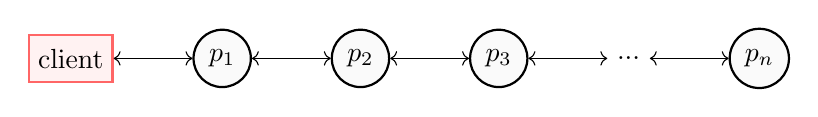
\begin{tikzpicture}[
squarednode/.style={rectangle, draw=red!60, fill=red!5, thick, minimum size=6mm},
roundnode/.style={circle, draw, thick, fill=black!2, minimum size=6mm},
ghostnode/.style={minimum size=5mm},
]
%Nodes
\node[squarednode]      (c0)       {client};
\node[roundnode]        (p1)       [right=of c0] {$p_1$};
\node[roundnode]        (p2)       [right=of p1] {$p_2$};
\node[roundnode]        (p3)       [right=of p2] {$p_3$};
\node[ghostnode]        (px)       [right=of p3] {$...$};
\node[roundnode]        (pn)       [right=of px] {$p_n$};

%Lines
\draw[<->] (c0.east) -- (p1.west);
\draw[<->] (p1.east) -- (p2.west);
\draw[<->] (p2.east) -- (p3.west);
\draw[<->] (p3.east) -- (px.west);
\draw[<->] (px.east) -- (pn.west);
\end{tikzpicture}
\end{center}
Each of the $p_i$ nodes here represents a queue cell which holds a value and are
linked together by bidirectional channels of type $\text{queue}_A$.  As
indicated by the type constructor $\&$, the first queue node $q_1$ first
receives either an $\textsf{ins}$ or $\textsf{del}$ label from the client. In
the case of an $\textsf{ins}$ label, $p_1$ receives a value $v$ of type $A$
(indicated by $\multimap$) from the client.  The $p_1$ node then sends an
$\textsf{ins}$ label to $p_2$ and forwards $v$ to it.  This forwarding process
repeats until the value reaches the end of the queue where a new queue cell
$p_{n+1}$ is allocated to store $v$. On the other hand, if $p_1$ receives a
$\textsf{del}$ label, the type constructor $\oplus$ requires that $p_1$ send
either $\textsf{none}$ or $\textsf{some}$.  The $\textsf{none}$ label is sent to
signify that the queue is empty and ready to terminate (indicated by $\End$).
The $\textsf{some}$ label is sent along with a value of type $A$ (indicated by $\otimes$)
which is the dequeued element. Finally, $p_1$ forwards its channel, connecting to
$p_2$, to the client so that the client may continue interacting with the rest of the queue.

It is clear from the example above that the session type $\textsf{queue}_A$ only lists
what operations a queue should support, but does not specify the expected behavior of
these operations. For instance, it does not specify that an $\textsf{ins}$ operation should
add an element to the back of the queue or that a $\textsf{del}$ operation should return the
element at the front of the queue. A correct implementation needs to maintain all of
these additional invariants not captured by the session type. In fact, due to the under
specification of the $\textsf{queue}_A$ type, it is possible to implement a ``queue''
which simply ignores all $\textsf{ins}$ messages and always returns $\textsf{none}$ on $\textsf{del}$.

% The refinement session types of Das et al.~\cite{das20} partially address this issue by
% using \emph{refinement types} to add more precision to session types. In this approach,
% the queue type is refined to the following:
% \begin{align*}
%   \textsf{queue}[n]_A \triangleq \&\{
%   \textsf{ins}: A \multimap \textsf{queue}[n+1]_A,
%   \textsf{del}: \oplus\{\textsf{none}: !\{n = 0\}. \End, \textsf{some}: !\{1 \leq n\}. A \otimes \textsf{queue}_A\}
%   \}
% \end{align*}
% Here, the type $\textsf{queue}[n]_A$ is parameterized by a natural number $n$ which represents
% the length of the queue. The $\textsf{ins}$ operation is refined to indicate that the length
% of the queue increases by one after an insertion. The $\textsf{del}$ operation is refined
% to indicate that the $\textsf{none}$ label may only be sent when the queue is empty (i.e. $n = 0$)
% and that the $\textsf{some}$ label may only be sent when the queue is non-empty (i.e. $1 \leq n$).
% While refinement session types are able to capture the length changes of the queue,
% ruling out many egregiously wrong implementations, they are still unable to capture the actual
% \emph{functional} behavior of the queue. For instance, a stack-like structure can be implemented
% with the above type as its length changes still comply with the refinements.

To address this issue, we develop \TLLC{}, a dependent session type system which
extends the Two-Level Linear dependent type theory (TLL)~\cite{fu23} with
session-typed concurrency. In \TLLC{}, one could define queues through the following
dependent session type:
\begin{alignat*}{2}
  &\textsf{queue} (\textit{xs} : \textsf{list}\ A) :=\ ?(\ell : \textsf{opr}). \Match\ \ell\ \With \\
  &\qquad\mid \textsf{ins}(v) \Rightarrow \textsf{queue}(\textsf{snoc}(xs, v)) \\
  &\qquad\mid \textsf{del} \Rightarrow
    \Match\ \textit{xs}\ \With
    \ (x :: xs') \Rightarrow\ !(\textsf{sing}\ x). !(\HC{\textsf{queue}(xs')}). \End
    \mid [] \Rightarrow \End
\end{alignat*}
Here, the type $\textsf{queue}(\textit{xs})$ is parameterized by a list $\textit{xs}$
which represents the current contents of the queue. Notice that the type no longer needs
the $\oplus$ and $\&$ type constructors to describe branching behavior. Instead, it uses
type-level pattern matching to inspect the label $\ell$ received from the client.
The \textsf{opr} type which $\ell$ inhabits is defined as a simple inductive type with
two constructors:
\begin{align*}
  \Inductive\ \textsf{opr} := \textsf{ins}: A \rightarrow \textsf{opr} \mid \textsf{del}: \textsf{opr}
\end{align*}
When a queue server receives an $\textsf{ins}(v)$ value, the type of the server becomes
$\textsf{queue}(\textsf{snoc}(xs, v))$ were $\textsf{snoc}$ appends $v$ to the end of $xs$.
Conversely, when a $\textsf{del}$ label is received, the type-level pattern matching on $xs$
enforces that if the queue is non-empty (i.e. $x :: xs'$ case), then the server must send
the front element $x$ of the queue to the client (indicated by the \emph{singleton type}
$\textsf{sing}\ x$) along with the channel $\HC{\textsf{queue}(xs')}$ connecting to the remainder
of the queue. If the queue is empty (i.e. $[]$ case), then the server simply terminates.

Given the \textsf{queue} protocol describe above, we can construct queue process nodes and
interact with them. The following signatures are of helper functions that wrap interactions with
the queue nodes into a convenient interface:
\begin{alignat*}{2}
  &\textsf{insert} &&: \forall \{xs : \textsf{list}\ A\}\;(x: A) \rightarrow \textsf{Queue}(xs) \rightarrow \textsf{Queue}(\textsf{snoc}(xs, x)) \\
  &\textsf{delete} &&: \forall \{x: A\}\;\{xs : \textsf{list}\ A\} \rightarrow
    \textsf{Queue}(x :: xs) \rightarrow \mcC (\textsf{sing}\ x \otimes \textsf{Queue}(xs)) \\
  &\textsf{free}   &&: \textsf{Queue}([]) \rightarrow \mcC(\textsf{unit})
\end{alignat*}
The \textsf{Queue} type here is a type alias for the \emph{channel type} of queues
(explained later in detail) and the $\mcC$ type constructor here is the \emph{concurrency monad}
which encapsulates concurrent computations. Notice in the signature of \textsf{insert} and
\textsf{delete} that there are dependent quantifiers surrounded by curly braces.
These are the \emph{implicit} quantifiers of TLL which indicate that the corresponding arguments
are ``ghost'' values used for type checking and erased prior to runtime. For our purposes here,
such ghost values are especially useful for \emph{relationally} specifying the expected
behaviors of queue interactions in terms of sequential list operations. For instance, the
signature of \textsf{insert} states that the queue obtained after inserting $x$ is related to
the original queue by the list operation $\textsf{snoc}$. Similarly, the signature of
\textsf{delete} states that deleting from a non-empty queue returns the front element $x$.
Even though neither of these $xs$ ghost values exist at runtime, they \emph{statically} ensure
that concurrent processes implementing these interfaces behave like actual queues, i.e.,
are first-in-first-out data structures. In a later section we will show how a generalized
map-reduce algorithm can be implemented and verified using similar techniques.


% It is important to note that these type-level pattern matches are \emph{static} and do not
% incur any runtime overhead. But most crucially, they guarantee that any concurrent program
% implementing this type behaves like an actual queue. Later we will show how a generalized
% map-reduce algorithm can be implemented and verified using similar techniques.

% Another important aspect of \TLLC{} is its ability to specify and reason about ``ghost'' messages
% in protocols using the computational irrelevancy machinery of TLL. Consider the session type encoding
% for an idealized Shannon cipher protocol:
% \begin{align*}
%   H(E, D) &\triangleq \forall \{k : \mcK\}\;\{m : \mcM\} \rightarrow D(k, E(k, m)) =_{\mcM} m
% \qquad\text{(correctness property)}
%   \\
%   \mcE(E, D) &\triangleq
%                !\{k : \mcK\}. !\{m : \mcM\}. !(c : \mcC). !\{p : H(E,D) \times (c =_\mcC E(k, m))\}. \End
% \end{align*}
% Given public encryption function $E: \mcK \times \mcM \rightarrow \mcC$ and
% decryption function $D: \mcK \times \mcC \rightarrow \mcM$, the protocol $\mcE(E,D)$ begins
% by sending \emph{implicit} messages as indicated by the curly braces: key $k$ of type $\mcK$
% and message $m$ of type $\mcM$. These implicit messages are \emph{ghosts} in the sense
% that they are only used for type checking and do not participate in runtime communication.
% During compilation, the sending and receiving of implicit messages are compiled to no-ops.
% Next, an \emph{explicit} ciphertext $c$ of type $\mcC$, indicated by round parenthesis,
% is sent to the client. Explicit messages are actual runtime messages which are sent and received.
% Finally, another implicit message $p$ is sent which is a proof object witnessing the
% correctness property of the protocol: $c$ is obtained by encrypting $m$ with key $k$.
% Observe that for the overall protocol, \emph{only} ciphertext $c$ will be sent at runtime while
% the other messages (secrets) are erased. The Shannon cipher protocol basically forces communicated messages
% to always be encrypted and prevents accidental leakage of plaintext.

Integrating session typed based concurrency into TLL is non-trivial due to the
fact that TLL is a dependently typed functional language. While prior
works~\cite{gay10,wadler12} have successfully combined \emph{classical} session
types with functional languages, its is well known that classical session types
do not easily support recursive session types~\cite{gay20} (needed to express
our \textsf{queue} type).  The main issue is that classical session types are
defined in terms of a \emph{dual} operator which does not easily commute with
recursive type definitions. The addition of arbitrary type-level computations
through dependent types further complicates this matter.  On the other hand,
\emph{intuitionistic} session types~\cite{caires10} eschew the dual operator and
define dual \emph{interpretations} of session types based their \emph{left} or
\emph{right} sequent rules.  Because intuitionistic session types do not rely on
a dual operator, they are able to support recursive session types without
commutativity issues. However, intuitionistic session types are often formulated
in the context of process calculi without a functional layer. To enjoy the
benefits of intuitionistic session types in a functional setting, we develop a
novel form of intuitionistic session types where we separate the notion of
\emph{protocols} from \emph{channel types}. The $\textsf{queue}(\textit{xs})$
type from before is, in actuality, a protocol whereas
$\HC{\textsf{queue}(\textit{xs})}$ is a channel type. In general, a channel type
is formed by applying the $\CH{\cdot}$ and $\HC{\cdot}$ type constructors to
protocols. These constructors provide dual interpretations to protocols,
allowing dual channels of the same protocol to be connected together. For
example, $!A. P$ would be interpreted dually as follows:
\begin{alignat*}{2}
  &\CH{!A. P}\quad &&(\textsf{send message of type } A) \\
  &\HC{!A. P}\quad &&(\textsf{receive message of type } A)
\end{alignat*}
Such channel types can be naturally included into the contexts of functional
type systems without needing to instrument the underlying language into a
sequent calculus formulation.  We believe our treatment of intuitionistic
session types is not specific to \TLLC{} and is widely applicable for
integrating intuitionistic session types with other functional languages.

In order to show that \TLLC{} ensures communication safety, we develop a process
calculus based concurrency semantics. Process configurations in the calculus are
collections of \TLLC{} programs interconnected by channels. At runtime,
individual processes are evaluated using the program semantics of base TLL. When
two processes at opposing ends (i.e. dually typed) of a channel are synchronized
and ready to communicate, the process level semantics transmits their messages
across the channel. We study the meta-theory of \TLLC{} and prove that it is
indeed sound at both the level of terms and at the level of process
configurations.

All lemmas and theorems reported in the this paper are formalized in
Rocq~\cite{coq}. All examples can be compiled into C programs using our prototype
compiler where concurrent processes are implemented using POSIX threads.  The
compiler implements advanced language features such dependent pattern matching
and functional in-place programming~\cite{lorenzen23} for linear types. Proofs,
source code, and examples are available in our git repository\footnote{\TODO}.

In summary, we make the following contributions:
\begin{itemize}
  \item We extend the Two-Level Linear dependent type theory (TLL) with session
        type based concurrency, forming the language of \TLLC{}. \TLLC{} inherits the
        strengths of TLL such as Martin-L\"{o}f style linear dependent types and the
        ability to control program erasure.
  \item We develop a novel formulation of intuitionistic session types
        through a clear separation of protocols and channel types. We believe
        this formulation to be widely applicable for integrating session types into
        other functional languages.
  \item We study the meta-theoretical properties of \TLLC{}. We show that
        \TLLC{}, as a term calculus, possesses desirable properties such as confluence and
        subject reduction and, as a process calculus, guarantees communication safety.
  \item The entire calculus, with its meta-theorems, is formalized in Rocq.
  \item We implement a prototype compiler which compiles \TLLC{} into safe and
        efficient C code.
\end{itemize}


%%% Local Variables:
%%% mode: LaTeX
%%% TeX-master: "main"
%%% End:


\section{Overview of Dependent Session Types}\label{sec:overview}
Session types in \TLLC{} are \emph{minimalistic} in design and yet surprisingly expressive
due to the presence of dependent types. Through examples, we provide an overview of
how dependent session types facilitate verified concurrent programming in \TLLC{}.

\subsection{Message Specification}\label{sec:message-specification}
An obvious, but important, use of dependent session types is the precise specification
of message properties communicated between parties. This is useful in practical network
systems where the content of messages may depend on the value of a prior request.
Consider the following protocol:
\begin{align*}
  !(\textit{sz}: \textsf{nat}).\
  ?(\textit{msg}: \textsf{bytes}).\ ?\{\textsf{sizeOf}(\textit{msg}) = \textit{sz}\}.\ \End
\end{align*}
Informally speaking, this protocol first expects a natural number \textit{sz} to be sent
followed by receiving a byte string \textit{msg}. In simple session type systems without
dependency, there would be no way of specifying the relationship between \textit{sz} and
\textit{msg}. However, dependent session types allow us to express relations between messages.
Notice in the third interaction expected by the protocol, the party sending \textit{msg} must
provide a \emph{proof} that the size of \textit{msg} is indeed \textit{sz} according to
an agreed upon \textsf{sizeOf} function. Finally, the protocol terminates with $\End$ and
communication ends. Notice that the proof here, as indicated by the curly braces, is a
\emph{ghost message}: it is used for type checking and erased prior to runtime. Even though
the proof does not participate in actual communication, the necessity for the send of
\textit{msg} to provide such a proof ensures that the protocol is followed correctly.

This example showcases the main primitives for constructing dependent protocols in
\TLLC{}: the $!(x : A).B$ and $?(x : A).B$ \emph{protocol actions}. The syntax of these
constructs take inspiration from binary session types~\cite{gay10,wadler12} and label
dependent session types~\cite{ldst}, however the meaning of these constructs in \TLLC{} is
subtly different. In prior works, the $!$ marker indicates that the channel is to send
and the $?$ marker indicates that the channel is to receive. In \TLLC{}, neither marker
expresses sending or receiving per se, but rather an abstract action that needs to be
interpreted through a \emph{channel type}. Hence, the description of the messaging protocol
above is stated to be informal. To assign a precise meaning to the protocol, we need to
view it through the lenses of channel types:
\begin{align*}
  &\CH{!(\textit{sz}: \textsf{nat}).\ ?(\textit{msg}: \textsf{bytes}).\ ?\{\textsf{sizeOf}(\textit{msg}) = \textit{sz}\}.\ \End} \\
  &\HC{!(\textit{sz}: \textsf{nat}).\ ?(\textit{msg}: \textsf{bytes}).\ ?\{\textsf{sizeOf}(\textit{msg}) = \textit{sz}\}.\ \End}
\end{align*}
Here, these two channel types are constructed using \emph{dual} channel type
constructors: $\CH{\cdot}$ and $\HC{\cdot}$.  The $\CH{\cdot}$ constructor
interprets $!$ as sending and $?$ as receiving while the $\HC{\cdot}$
constructor interprets $!$ as receiving and $?$ as sending. In other words, dual
channel types interpret protocol actions in opposite ways. These constructors act similarly
to the duality of left and right rules for intuitionistic session types~\cite{caires10}.
Unlike intuitionistic session types which require the base type system to be
based on sequent calculus, our channel types can be integrated into the type
systems of functional languages so long as linear types are supported.

\subsection{Dependent Ghost Secrets}
Dependent ghost messages have interesting applications when it comes to message specification.
Consider the following encoding of a idealized Shannon cipher protocol:
\begin{align*}
  H(E, D) &:= \forall \{k : \mcK\}\;\{m : \mcM\} \rightarrow D(k, E(k, m)) =_{\mcM} m
\qquad\text{(correctness property)}
  \\
  \mcE(E, D) &:=\ !\{k : \mcK\}.\ !\{m : \mcM\}.\ !(c : \mcC).\ !\{H(E,D) \times (c =_\mcC E(k, m))\}.\ \End
\end{align*}
Given public encryption and decryption functions
$E: \mcK \times \mcM \rightarrow \mcC$ and
$D: \mcK \times \mcC \rightarrow \mcM$ respectively, the protocol $\mcE(E,D)$
begins by sending ghost messages: key $k$ of type $\mcK$ and message $m$ of type
$\mcM$.  Next, the ciphertext $c$ of type $\mcC$, indicated by round
parenthesis, is actually sent to the client. Finally, the last ghost message
sent is a proof object witnessing the correctness property of the
protocol: $c$ is obtained by encrypting $m$ with key $k$.  Observe that for the
overall protocol, \emph{only} ciphertext $c$ will be sent at runtime while the
other messages (secrets) are erased. The Shannon cipher protocol basically
forces communicated messages to always be encrypted and prevents the accidental
leakage of plaintext.

It is important to note that ghost messages and proof specifications, by
themselves, are \emph{not} sufficient to guaranteeing semantic security.
An adversary can simply use a different programming language and circumvent the
proof obligations imposed by \TLLC{}. However, these obligations are useful in
ensuring that honest parties correctly follow \emph{trusted} protocols to defend
against attackers. For example, in the Shannon cipher protocol above, an honest
party is required by the type system to send a ciphertext that is indeed encrypted
from the (trusted) algorithm $E$.

Another, more concrete, example of using ghost messages to specify secrets is the
Diffie-Hellman key exchange~\cite{DH76} protocol defined as follows:
\begin{align*}
  \textsf{DH}(p\ g: \textsf{int})
  :=\ & !\{a: \textsf{int}\}.\ !(A: \textsf{int}).\ !\{A = \textsf{powm}(g, a, p)\}.\\
      & ?\{b: \textsf{int}\}.\ ?(B: \textsf{int}).\ ?\{B = \textsf{powm}(g, b, p)\}.\ \End
\end{align*}
The \textsf{DH} protocol is parameterized by publicly known integers $p$ and $g$.
Without loss of generality, we refer to the message sender for the first row of the
protocol as Alice and the message sender for the second row as Bob. From Alice's
perspective, she first sends her secret value $a$ as a dependent ghost message to
initialize her half of the protocol. Next, her public value $A$ is sent as a real
message to Bob along with a proof that $A$ is correctly computed from values $p, g$ and $a$
(using modular exponentiation \textsf{powm}). At this point, Alice has finished sending
messages and waits for message from Bob to complete the key exchange. She first
``receives'' Bob's secret $b$ as a ghost message which initializes Bob's half of the
protocol. Later, Bob' public value $B$ is received as a real message along with a proof
that $B$ is correctly computed from $p, g$ and $b$. Notice that between Alice and Bob,
the only the real messages $A$ and $B$ will be exchanged at runtime. The secret values
$a$ and $b$ and the correctness proofs are all ghost message that are erased prior to
runtime. Basically, the \textsf{DH} protocol forces communication between Alice and Bob
to be encrypted and maintain secrecy at runtime.

\vspace{-0.4em}
\begin{center}
\begin{minipage}{0.45\textwidth}
\begingroup
\small
\addtolength{\jot}{-0.25em}
\begin{alignat*}{4}
  &\Def\ \textsf{Alice}\ (a\ p\ g: \textsf{int})\ (c : \CH{\textsf{DH}(p,g)}) \\
  &: \CM{\textsf{unit}} := \\
  &\quad\Let\ c \Leftarrow \Send\ c\ \{ a \}\ \In \\
  &\quad\Let\ c \Leftarrow \Send\ c\ (\textsf{powm}(g, a, p))\ \In \\
  &\quad\Let\ c \Leftarrow \Send\ c\ \{\textsf{refl}\}\ \In \\
  &\quad\Let\ \langle{\{b\}, c}\rangle \Leftarrow \Recv\ c\ \In \\
  &\quad\Let\ \langle{B, c}\rangle \Leftarrow \Recv\ c\ \In \\
  &\quad\Let\ \langle{\{\textit{pf}\}, c}\rangle \Leftarrow \Recv\ c\ \In \\
  &\quad\Close(c)
\end{alignat*}
\endgroup
\end{minipage}
\begin{minipage}{0.5\textwidth}
\begingroup
\small
\addtolength{\jot}{-0.25em}
\begin{alignat*}{4}
  &\Def\ \textsf{Bob}\ (b\ p\ g: \textsf{int})\ (c : \HC{\textsf{DH}(p,g)}) \\
  &: \CM{\textsf{unit}} := \\
  &\quad\Let\ \langle{\{a\}, c}\rangle \Leftarrow \Recv\ c\ \In \\
  &\quad\Let\ \langle{A, c}\rangle \Leftarrow \Recv\ c\ \In \\
  &\quad\Let\ \langle{\{\textit{pf}\}, c}\rangle \Leftarrow \Recv\ c\ \In \\
  &\quad\Let\ c \Leftarrow \Send\ c\ \{ b \}\ \In \\
  &\quad\Let\ c \Leftarrow \Send\ c\ (\textsf{powm}(g, b, p))\ \In \\
  &\quad\Let\ c \Leftarrow \Send\ c\ \{\textsf{refl}\}\ \In \\
  &\quad\Wait(c)
\end{alignat*}
\endgroup
\end{minipage}
\end{center}
\vspace{0.5em}

The \textsf{DH} key exchange protocol can be implemented through two simple monadic
programs \textsf{Alice} and \textsf{Bob} as shown above. The $\mcC$ type constructor
here is the concurrency monad for integrating the \emph{effect} of concurrent
communication with the \emph{pure} functional core of \TLLC{}. There are two kinds of
\textsf{send} (and respectively \textsf{recv}) operations at play here.
The first kind, indicated by $\textsf{send}\ c\ \{v\}$ is for sending a ghost message
$v$ on channel $c$. After type checking, these ghost sends are compiled to no-ops
to that they do not participate in runtime communication. The second kind, indicated by
$\textsf{send}\ c\ (v)$, is for sending a real message $v$ on channel $c$. These
real sends are compiled to actual messages in the generated code. Finally, the
\textsf{close} and \textsf{wait} operations synchronize the termination of the protocol.
Notice that the duality of channel types $\CH{\textsf{DH}(p,g)}$ and $\HC{\textsf{DH}(p,g)}$
ensure that every send in \textsf{Alice} is matched by a corresponding receive in
\textsf{Bob} and vice versa. Moreover, \textsf{Alice} and \textsf{Bob} are enforced by the
type checker to correctly carry out the Diffie-Hellman key exchange.

%%% Local Variables:
%%% mode: LaTeX
%%% TeX-master: "main"
%%% End:


\section{Relational Verification via Dependent Session Types}\label{sec:relational}
Earlier in the introduction section, we showed a sketch of how dependent session types
can be used for certified concurrent programming through the example of a concurrent queue.
In this section, we provide a detailed account of how we can use dependent session types
to construct a generic map-reduce system. Similarly to the queue example, we will verify
the correctness of the map-reduce system by relating it to sequential operations on trees.

The first step in constructing the map-reduce system is to define the kinds of operations
that can be performed by the system.
\begingroup
\small
\addtolength{\jot}{-0.2em}
\begin{align*}
  \Inductive\ \textsf{opr}(A : \Un) :=\ &\textsf{Free}  : \textsf{opr}(A) \\
  \mid\ &\textsf{Map}   : \forall \{B : \Un\}\ (f : A \rightarrow B) \rightarrow \textsf{opr}(A) \\
  \mid\ &\textsf{Reduce}: \forall \{B : \Un\}\ (f : A \rightarrow B)\ (g : B \rightarrow B \rightarrow B) \rightarrow \textsf{opr}(A)
\end{align*}
\endgroup

%%% Local Variables:
%%% mode: LaTeX
%%% TeX-master: "main"
%%% End:


\section{Formal Theory of Dependent Session Types}\label{sec:theory}
\subsection{Core TLL}
In this section, we give a brief summary of the Two-Level Linear dependent type theory (TLL)~\cite{fu23}. 
TLL is a dependent type theory that combines 
Martin-L\"{o}f-style dependent types~\cite{martinlof} 
with linear types~\cite{girard,wadler1990}. 
Notably, TLL supports \emph{essential linearity}~\cite{luo} through the use of
a stratified ``two-level'' typing system: the \emph{logical} level and the \emph{program} level. 
The typing judgments of the two levels are written as follows:
\begin{center}
\vspace{0.5em}
\begin{tikzpicture}[
    node distance=2.4cm,
    >=stealth, auto,
    every state/.style={rectangle, draw, rounded corners}
]
\node[state, fill=blue!5] (l)                {\small$\Gamma \vdash m : A\ \text{(Logical Typing)}$};
\node[state, fill=red!5]  (p) [right=of l]   {\small$\Gamma ; \Delta \vdash m : A\ \text{(Program Typing)}$};
\path[-latex,transform canvas={yshift=+1.5ex}] (l.east) edge node {\footnotesize{provides types}} (p.west);
\path[-latex,transform canvas={yshift=-1.5ex}] (p.west) edge node {\footnotesize{subjects to verify}} (l.east);
\end{tikzpicture}
\vspace{0.5em}
\end{center}

First, the \emph{logical} level is a standard dependent type system that supports unrestricted 
usage of types and terms. The primary purpose of the logical level is to provide typing rules
for types which will be used at the logical level. For example, the rules for dependent 
function type ($\Pi$-types) formation are defined at the logical level as follows:
\begin{mathpar}
  \inferrule[Explicit-Fun]
  { \Gamma \vdash A : s \\
    \Gamma, x : A \vdash B : r }
  { \Gamma \vdash \PiR{t}{x : A}{B} : t }

  \inferrule[Implicit-Fun]
  { \Gamma \vdash A : s \\
    \Gamma, x : A \vdash B : r }
  { \Gamma \vdash \PiI{t}{x : A}{B} : t }
\end{mathpar}
The symbols $s, r, t$ range over the \emph{sorts} of type universes, i.e. 
$\Un$ or $\Ln$. These sorts are used to classify types into two categories: 
unrestricted types ($A : \Un$) and linear types ($A : \Ln$).
Program level terms which inhabit unrestricted types can be freely duplicated or discarded,
while those which inhabit linear types must be used exactly once.
Note that this usage restriction is \emph{not} enforced at the logical level
as the logical level typing judgment is completely structural.
This is safe because the logical level will never be executed at runtime and 
is only used for type checking and verification. Thus, multiple uses of
a linear resource at the logical level will not lead to any runtime errors.

At the program level, the typing judgment $\Gamma ; \Delta \vdash m : A$ is used to
exclusively type \emph{terms}. In other words, no rules for forming types are defined
at the program level. All the types used in $\Gamma$, $\Delta$, $m$ and $A$ must be well-formed
according to the logical level typing judgment. This typing judgment possesses two contexts:
$\Gamma$ of all variables in scope, and $\Delta$ of all variables that are computationally relevant
in program $m$. Context $\Delta$ is crucial for enforcing linearity at the program level.
For example, consider the $\lambda$-abstraction rules:
\begin{mathpar}
  \inferrule[Explicit-Lam]
  { \Gamma, x : A ; \Delta, x :_s A \vdash m : B \\ 
    \Delta \triangleright t }
  { \Gamma ; \Delta \vdash \lamR{t}{x : A}{m} : \PiR{t}{x : A}{B} }

  \inferrule[Implicit-Lam]
  { \Gamma, x : A ; \Delta \vdash m : B \\
    \Delta \triangleright t }
  { \Gamma ; \Delta \vdash \lamI{t}{x : A}{m} : \PiI{t}{x : A}{B} }
\end{mathpar}
In \textsc{Explicit-Lam}, we can see that the bound variable $x$ is added to
both contexts $\Gamma$ and $\Delta$. This indicates that $x$ is a variable which
can be used both logically (in types and ghost values) through $\Gamma$, and
computationally (in real values) through $\Delta$. On the other hand, in the
\textsc{Implicit-Lam} rule, $x$ is only added to $\Gamma$ but not $\Delta$.
This indicates that $x$ is a ghost variable which can only be used logically.
A ubiquitous example of ghost variables are type parameters in polymorphic functions.
For example, the polymorphic identity function can be implemented as
\begin{align*}
  \lamI{\Un}{A : \Un}{\lamR{\Un}{x : A}{x}}
\end{align*}
which has the type $\PiI{\Un}{A : \Un}{\PiR{\Un}{x : A}{A}}$.
Arguments to implicit functions are typed at the logical level, thus
allowing polymorphic functions to be instantiated with a type as an argument.
Additionally, as demonstrated in the examples of prior sections,
ghost variables also facilitate program verification by statically describing 
abstractions and invariants of program states.

In the two $\lambda$-abstraction rules above, 
the premise $\Delta \triangleright t$ is a simple side condition that states: if
$t = \Un$, then all variables in $\Delta$ must be unrestricted. In other words,
the $\lambda$-abstractions that can be applied unrestrictedly (with $t = \Un$)
are not allowed to capture linearly typed variables from $\Delta$. This is
similar to the restriction imposed on closures implementing the $\textsf{Fn}$
trait (i.e. those that can be called multiple times) in Rust~\cite{rust} where
capturing of mutable references is prohibited. If such a restriction is not
imposed, then evaluating a $\lambda$-abstraction (that captures a linear
variable) twice may lead to unsafe memory accesses such as double frees or
use-after-frees.

The application rules for both explicit and implicit functions are as follows:
\begin{mathpar}
  \inferrule[Explicit-App]
  { \Gamma ; \Delta_1 \vdash m : \PiR{t}{x : A}{B} \\ 
    \Gamma ; \Delta_2 \vdash n : A }
  { \Gamma ; \Delta_1 \dotcup \Delta_2 \vdash \appR{m}{n} : B[n/x] }

  \inferrule[Implicit-App]
  { \Gamma ; \Delta \vdash m : \PiI{t}{x : A}{B} \\ 
    \Gamma \vdash n : A }
  { \Gamma ; \Delta \vdash \appI{m}{n} : B[n/x] }
\end{mathpar}
In \textsc{Explicit-App}, the argument $n$ is a real value which must be typed
at the program level. The $\dotcup$ operator merges the two program context
$\Delta_1$ and $\Delta_2$ by contracting unrestricted variables and requiring
that linear variables be disjoint, thus preventing the sharing of linear
resources. In \textsc{Implicit-App}, the argument $n$ is a ghost value that is
typed at the logical level. Due to the fact that ghost values are erased prior
to runtime, the program context $\Delta$ in the conclusion only tracks the
computationally relevant variables used in $m$. Notice how in \textsc{Explicit-App}, 
the argument $n$ is substituted into the return type $B$. This allows types to depend 
on program level terms regardless of whether they are of linear or unrestricted types.

\paragraph{\textbf{Usage vs Uniqueness}}
Compared to other linear dependent type
theories~\cite{qtt,nothing,llf,vakar14,luo} which only enforce the linear
\emph{usage} of resources, the TLL type system prevents the \emph{sharing} of
linear resources as well. This is similar to the subtle difference between
linear logic~\cite{girard} and bunched implications~\cite{ohearn99,ohearn03}. 
Consider a linear function $f$, in the aforementioned dependent type theories,
of some type $A \multimap B$. When function $f$ is applied to some argument $v$
of type $A$, the argument $v$ is guaranteed to be used exactly once in the 
\emph{body} of $f$. Notice that this notion of linearity does not preclude the
possibility of sharing $v$ with other functions or threads outside of $f$. In
contrast, the shared interpretation of linearity, as described by
O'Hearn~\cite{ohearn03}, require that $v$ be a unique resource which is
exclusively owned by $f$. In other words, $v$ cannot be shared with any other
functions or threads outside of $f$. Wadler, in his seminal
work~\cite{wadler1991}, also made a similar distinction between \emph{linearity}
and \emph{uniqueness} in the context of functional programming, coining the term
\emph{steadfast types} to refer to type systems that enforce both linearity and
uniqueness. In the context of concurrency, the steadfast type system of TLL
makes it especially suitable for integration with session types: linear usage
prevents replaying of communication protocols and uniqueness prevents multiple
threads from simultaneously accessing the same communication channel.

\subsection{Dependent Session Types of \TLLC{}}
In this section, we formally present the dependent session types of \TLLC{}.

\paragraph{\textbf{Protocols and Channel Types}}
As touched on in \Cref{sec:message-specification}, intuitionistic session types
of \TLLC{} are decoupled into \emph{protocols} and \emph{channel types}. 
The rule for forming protocols is as follows:
\begin{mathpar}
  \inferrule[Proto] 
  { \Gamma \vdash }
  { \Gamma \vdash \Proto : \Un }

  \inferrule[Explicit-Action]
  { \Gamma, x : A \vdash B : \Proto }
  { \Gamma \vdash \ActR{\rho}{x : A}{B} : \Proto }

  \inferrule[Implicit-Action]
  { \Gamma, x : A \vdash B : \Proto }
  { \Gamma \vdash \ActI{\rho}{x : A}{B} : \Proto }

  \inferrule[End]
  { \Gamma \vdash }
  { \Gamma \vdash \End : \Proto }

  \text{where } \rho \in \{!, ?\}
\end{mathpar}
Here, the \textsc{Proto} rule introduces the \Proto{} type which is the type of all protocols. 
Note that \Proto{} is an unrestricted type, thus protocols can be freely duplicated or discarded.
The \textsc{Explicit-Action} and \textsc{Implicit-Action} rules form dependent protocols which 
inhabit the \Proto{} type. The \textsc{End} rule marks the termination of a protocol.

\begin{mathpar}
  \inferrule[ChType]
  { \Gamma \vdash A : \Proto }
  { \Gamma \vdash \CH{A} : \Ln }

  \inferrule[Ch]
  { \Gamma ; \Delta \vdash \\ 
    \epsilon \vdash A : \Proto \\ 
    \Delta \triangleright \Un }
  { c :_\Ln \CH{A} ; \Gamma ; \Delta \vdash c : \CH{A} }
\end{mathpar}

\paragraph{\textbf{Concurrency Monad}}

\section{Semantics and Meta-Theory}\label{sec:semantics}
In this section, we present the operational semantics of \TLLC{}. 
Similarly to the typing rules, we organize the presentation of the semantics
into the logical level, program level, and process level.

\subsection{Logical Level}\label{appendix:logical-semantics}
The semantics of the logical level is defined in terms of the 
\emph{parallel reduction} relation $m \Rightarrow m'$. This relation allows 
multiple redexes to be reduced simultaneously.

\paragraph{\textbf{Core Reduction}}
The parallel reduction for core functional terms is defined as follows:
\begin{mathpar}\footnotesize
  \inferrule[PStep-Var]
  { }
  { x \Rightarrow x }

  \inferrule[PStep-Sort]
  { }
  { s \Rightarrow s }

  \inferrule[PStep-Explicit-Fun]
  { A \Rightarrow A' \\ B \Rightarrow B' }
  { \PiR{s}{x : A}{B} \Rightarrow \PiR{s}{x : A'}{B'} }

  \inferrule[PStep-Implicit-Fun]
  { A \Rightarrow A' \\ B \Rightarrow B' }
  { \PiI{s}{x : A}{B} \Rightarrow \PiI{s}{x : A'}{B'} }

  \inferrule[PStep-Explicit-Lam]
  { A \Rightarrow A' \\ B \Rightarrow B' }
  { \lamR{s}{x : A}{B} \Rightarrow \lamR{s}{x : A'}{B'} }

  \inferrule[PStep-Implicit-Lam]
  { A \Rightarrow A' \\ B \Rightarrow B' }
  { \lamI{s}{x : A}{B} \Rightarrow \lamI{s}{x : A'}{B'} }

  \inferrule[PStep-Explicit-App]
  { m \Rightarrow m' \\ n \Rightarrow n' }
  { \appR{m}{n} \Rightarrow \appR{m'}{n'} }

  \inferrule[PStep-Implicit-App]
  { m \Rightarrow m' \\ n \Rightarrow n' }
  { \appI{m}{n} \Rightarrow \appI{m'}{n'} }

  \inferrule[PStep-Explicit-$\beta$]
  { m \Rightarrow m' \\ n \Rightarrow n' }
  { \appR{(\lamR{s}{x : A}{m})}{n} \Rightarrow m'[n'/x] }

  \inferrule[PStep-Implicit-$\beta$]
  { m \Rightarrow m' \\ n \Rightarrow n' }
  { \appI{(\lamI{s}{x : A}{m})}{n} \Rightarrow m'[n'/x] }

  \inferrule[PStep-Explicit-Sum]
  { A \Rightarrow A' \\ B \Rightarrow B' }
  { \SigR{s}{x : A}{B} \Rightarrow \SigR{s}{x : A'}{B'} }

  \inferrule[PStep-Implicit-Sum]
  { A \Rightarrow A' \\ B \Rightarrow B' }
  { \SigI{s}{x : A}{B} \Rightarrow \SigI{s}{x : A'}{B'} }

  \inferrule[PStep-Explicit-Pair]
  { m \Rightarrow m' \\ n \Rightarrow n' }
  { \pairR{m}{n}{s} \Rightarrow \pairR{m'}{n'}{s} }

  \inferrule[PStep-Implicit-Pair]
  { m \Rightarrow m' \\ n \Rightarrow n' }
  { \pairI{m}{n}{s} \Rightarrow \pairI{m'}{n'}{s} }

  \inferrule[PStep-SumElim]
  { A \Rightarrow A' \\ m \Rightarrow m' \\ n \Rightarrow n' }
  { \SigElim{[z]A}{m}{[x,y]n} \Rightarrow \SigElim{[z]A'}{m'}{[x,y]n'} }

  \inferrule[PStep-Explicit-PairElim]
  { m_1 \Rightarrow m_1' \\ m_2 \Rightarrow m_2' \\ n \Rightarrow n' }
  { \SigElim{[z]A}{\pairR{m_1}{m_2}{s}}{[x,y]n} \Rightarrow n'[m_1/x,m_2/y] }

  \inferrule[PStep-Implicit-PairElim]
  { m_1 \Rightarrow m_1' \\ m_2 \Rightarrow m_2' \\ n \Rightarrow n' }
  { \SigElim{[z]A}{\pairI{m_1}{m_2}{s}}{[x,y]n} \Rightarrow n'[m_1/x,m_2/y] }
\end{mathpar}

\paragraph{\textbf{Data Reduction}}
The parallel reduction for data terms is defined as follows:
\begin{mathpar}\footnotesize
  \inferrule[PStep-Unit]
  { }
  { \unit \Rightarrow \unit }

  \inferrule[PStep-UnitVal]
  { }
  { \ii \Rightarrow \ii }

  \inferrule[PStep-Bool]
  { }
  { \Bool \Rightarrow \Bool }

  \inferrule[PStep-True]
  { }
  { \bTrue \Rightarrow \bTrue }

  \inferrule[PStep-False]
  { }
  { \bFalse \Rightarrow \bFalse }

  \inferrule[PStep-BoolElim]
  { A \Rightarrow A' \\
    m \Rightarrow m' \\
    n_1 \Rightarrow n_1' \\
    n_2 \Rightarrow n_2' }
  { \boolElim{[z]A}{m}{n_1}{n_2} \Rightarrow \boolElim{[z]A'}{m'}{n_1'}{n_2'} }

  \inferrule[PStep-TrueElim]
  { n_1 \Rightarrow n_1' }
  { \boolElim{[z]A}{\bTrue}{n_1}{n_2} \Rightarrow n_1' }

  \inferrule[PStep-FalseElim]
  { n_2 \Rightarrow n_2' }
  { \boolElim{[z]A}{\bFalse}{n_1}{n_2} \Rightarrow n_2' }
\end{mathpar}

\paragraph{\textbf{Monadic Reduction}}
The parallel reduction for monadic terms is defined as follows:
\begin{mathpar}\footnotesize
  \inferrule[PStep-$\mcC$Type]
  { A \Rightarrow A' }
  { \CM{A} \Rightarrow \CM{A'} }

  \inferrule[PStep-Return]
  { m \Rightarrow m' }
  { \return{m} \Rightarrow \return{m'} }

  \inferrule[PStep-Bind]
  { m \Rightarrow m' \\ n \Rightarrow n' }
  { \letin{x}{m}{n} \Rightarrow \letin{x}{m'}{n'} }

  \inferrule[PStep-ReturnBind]
  { m \Rightarrow m' \\ n \Rightarrow n' }
  { \letin{x}{\return{m}}{n} \Rightarrow n'[m'/x] }
\end{mathpar}
\clearpage

\paragraph{\textbf{Session Reduction}}
The parallel reduction for protocols, channels and concurrency primitives are defined as follows:
\begin{mathpar}\footnotesize
  \inferrule[PStep-Proto]
  { }
  { \Proto \Rightarrow \Proto }

  \inferrule[PStep-End]
  { }
  { \End \Rightarrow \End }

  \inferrule[PStep-RecProto]
  { A \Rightarrow A' \\ m \Rightarrow m' }
  { \fix{x : A}{m} \Rightarrow \fix{x : A'}{m'} }

  \inferrule[PStep-RecUnfold]
  { A \Rightarrow A' \\ m \Rightarrow m' }
  { \fix{x : A}{m} \Rightarrow m'[(\fix{x : A'}{m'})/x] }

  \inferrule[PStep-Explicit-Action]
  { A \Rightarrow A' \\ B \Rightarrow B' }
  { \ActR{\rho}{x : A}{B} \Rightarrow \ActR{\rho}{x : A'}{B'} }

  \inferrule[PStep-Implicit-Action]
  { A \Rightarrow A' \\ B \Rightarrow B' }
  { \ActI{\rho}{x : A}{B} \Rightarrow \ActI{\rho}{x : A'}{B'} }

  \inferrule[PStep-CH]
  { A \Rightarrow A' }
  { \CH{A} \Rightarrow \CH{A'} }

  \inferrule[PStep-HC]
  { A \Rightarrow A' }
  { \HC{A} \Rightarrow \HC{A'} }

  \inferrule[PStep-Channel]
  { }
  { c \Rightarrow d }

  \inferrule[PStep-Fork]
  { A \Rightarrow A' \\ m \Rightarrow m' }
  { \fork{x : A}{m} \Rightarrow \fork{x : A'}{m'} }

  \inferrule[PStep-Explicit-Send]
  { m \Rightarrow m' }
  { \sendR{m} \Rightarrow \sendR{m'} }

  \inferrule[PStep-Implicit-Send]
  { m \Rightarrow m' }
  { \sendI{m} \Rightarrow \sendI{m'} }

  \inferrule[PStep-Explicit-Recv]
  { m \Rightarrow m' }
  { \recvR{m} \Rightarrow \recvR{m'} }

  \inferrule[PStep-Implicit-Recv]
  { m \Rightarrow m' }
  { \recvI{m} \Rightarrow \recvI{m'} }

  \inferrule[PStep-Close]
  { m \Rightarrow m' }
  { \close{m} \Rightarrow \close{m'} }

  \inferrule[PStep-Wait]
  { m \Rightarrow m' }
  { \wait{m} \Rightarrow \wait{m'} }
\end{mathpar}

\paragraph{\textbf{Convertibility Relation}}
The convertibility relation $A \simeq B$ is the reflexive, symmetric and
transitive closure of the parallel reduction relation. It can be inductively
defined as follows:
\begin{mathpar}
  \inferrule[Conv-Refl]
  { }
  { A \simeq A }

  \inferrule[Conv-PStep]
  { A \simeq B \\ 
    B \Rightarrow C }
  { A \simeq C }

  \inferrule[Conv-PStep-Rev]
  { A \simeq B \\ 
    C \Rightarrow B }
  { A \simeq C }
\end{mathpar}
Note that the program level \textsc{Conversion} rule (\Cref{appendix:program-typing}) 
also uses this convertibility relation.
\clearpage

\subsection{Program Level}\label{appendix:program-semantics}
The semantics of the program level is defined in terms of a small-step reduction
relation $m \Leadsto m'$. Unlike the logical level which has a non-deterministic
reduction strategy, the program level follows call-by-value evaluation.
Arguments are fully evaluated before substitution into functions.

\paragraph{\textbf{Core Reduction}}
The small-step reduction for core functional terms is defined as follows:
\begin{mathpar}\footnotesize
  \inferrule[Step-Explicit-App$_1$]
  { m \Leadsto m' }
  { \appR{m}{n} \Leadsto \appR{m'}{n} }

  \inferrule[Step-Explicit-App$_2$]
  { n \Leadsto n' }
  { \appR{m}{n} \Leadsto \appR{m}{n'} }

  \inferrule[Step-Implicit-App$_1$]
  { m \Leadsto m' }
  { \appI{m}{n} \Leadsto \appI{m'}{n} }
  
  \inferrule[Step-Explicit-$\beta$]
  { }
  { \appR{(\lamR{s}{x : A}{m})}{v} \Leadsto m[v/x] }

  \inferrule[Step-Implicit-$\beta$]
  { }
  { \appI{(\lamI{s}{x : A}{m})}{n} \Leadsto m[n/x] }

  \inferrule[Step-Explicit-Pair$_1$]
  { m \Leadsto m' }
  { \pairR{m}{n}{s} \Leadsto \pairR{m'}{n}{s} }

  \inferrule[Step-Explicit-Pair$_2$]
  { n \Leadsto n' }
  { \pairR{m}{n}{s} \Leadsto \pairR{m}{n'}{s} }

  \inferrule[Step-Implicit-Pair$_2$]
  { n \Leadsto n' }
  { \pairI{m}{n}{s} \Leadsto \pairI{m}{n'}{s} }

  \inferrule[Step-SumElim$_1$]
  { m \Leadsto m' }
  { \SigElim{[z]A}{m}{[x,y]n} \Leadsto \SigElim{[z]A}{m'}{[x,y]n} }

  \inferrule[Step-Explicit-PairElim]
  { }
  { \SigElim{[z]A}{\pairR{u}{v}{s}}{[x,y]n} \Leadsto n[u/x,v/y] }

  \inferrule[Step-Implicit-PairElim]
  { }
  { \SigElim{[z]A}{\pairI{m}{v}{s}}{[x,y]n} \Leadsto n[m/x,v/y] }
\end{mathpar}

\paragraph{\textbf{Data Reduction}}
The small-step reduction for data terms is defined as follows:
\begin{mathpar}\small
  \inferrule[Step-BoolElim]
  { m \Leadsto m' }
  { \boolElim{[z]A}{m}{n_1}{n_2} \Leadsto \boolElim{[z]A}{m'}{n_1}{n_2} }

  \inferrule[Step-TrueElim]
  { }
  { \boolElim{[z]A}{\bTrue}{n_1}{n_2} \Leadsto n_1 }

  \inferrule[Step-FalseElim]
  { }
  { \boolElim{[z]A}{\bFalse}{n_1}{n_2} \Leadsto n_2 }
\end{mathpar}

\paragraph{\textbf{Monadic Reduction}}
The small-step reduction for monadic terms is defined as follows:
\begin{mathpar}\small
  \inferrule[Step-Return]
  { m \Leadsto m' }
  { \return{m} \Leadsto \return{m'} }

  \inferrule[Step-Bind]
  { m \Leadsto m' }
  { \letin{x}{m}{n} \Leadsto \letin{x}{m'}{n} }

  \inferrule[Step-ReturnBind]
  { v~\val }
  { \letin{x}{\return{v}}{n} \Leadsto n[v/x] }
\end{mathpar}

\paragraph{\textbf{Session Reduction}}
The small-step reduction for session terms is defined as follows:
\begin{mathpar}\small
  \inferrule[Step-Explicit-Send]
  { m \Leadsto m' }
  { \sendR{m} \Leadsto \sendR{m'} }

  \inferrule[Step-Implicit-Send]
  { m \Leadsto m' }
  { \sendI{m} \Leadsto \sendI{m'} }

  \inferrule[Step-Explicit-Recv]
  { m \Leadsto m' }
  { \recvR{m} \Leadsto \recvR{m'} }

  \inferrule[Step-Implicit-Recv]
  { m \Leadsto m' }
  { \recvI{m} \Leadsto \recvI{m'} }

  \inferrule[Step-Close]
  { m \Leadsto m' }
  { \close{m} \Leadsto \close{m'} }

  \inferrule[Step-Wait]
  { m \Leadsto m' }
  { \wait{m} \Leadsto \wait{m'} }
\end{mathpar}
\clearpage

\subsection{Process Level}\label{appendix:process-semantics}
The semantics of the process level is defined in terms of a small-step reduction
relation $P \Rrightarrow Q$. This relation is what gives \TLLC{} its concurrent
behavior. Before we present the reduction rules, we first define the notion of
\emph{structural congruence} $\equiv$ which identifies processes that are
the same up to reordering of parallel components and renaming of bound channels.

\paragraph{\textbf{Structural Congruence}}
The structural congruence relation $\equiv$ is defined as follows:
\begin{mathpar}\small
  P \mid Q \equiv Q \mid P 

  O \mid (P \mid Q) \equiv (O \mid P) \mid Q

  P \mid \proc{\return{\ii}} \equiv P
  \\
  \scope{cd}{P} \mid Q \equiv \scope{cd}{(P \mid Q)}

  \scope{cd}{P} \equiv \scope{dc}{P}

  \scope{cd}{\scope{c'd'}{P}} \equiv \scope{c'd'}{\scope{cd}{P}}
\end{mathpar}

\paragraph{\textbf{Process Reduction}}
The small-step reduction for processes is defined as follows:

\vspace{1em}
\begin{small}
\begin{tabular}{l L}
  (\textsc{Proc-Fork}) &
    \proc{\letin{x}{\fork{y : A}{m}}{n}}
    \Rrightarrow
    \scope{cd}{(\proc{n[c/x]} \mid \proc{m[d/y]})} 
  \\
  (\textsc{Proc-End}) 
    &\scope{cd}{(\proc{\letin{x}{\close{c}}{m}} \mid \proc{\letin{y}{\wait{d}}{n}})} \\
    &\quad\Rrightarrow 
     \proc{\letin{x}{\return{\ii}}{m}} \mid \proc{\letin{y}{\return{\ii}}{n}} 
  \\
  (\textsc{Proc-Com}) 
    &\scope{cd}{(\proc{\letin{x}{\appR{\sendR{c}}{v}}{m}} \mid \proc{\letin{y}{\recvR{d}}{n}})} \\
    &\quad\Rrightarrow 
     \scope{cd}{(\proc{\letin{x}{\return{c}}{m}} \mid \proc{\letin{y}{\return{\pairR{v}{d}{\Ln}}}{n}})}
  \\
  (\textsc{Proc-\underline{Com}}) 
    &\scope{cd}{(\proc{\letin{x}{\appI{\sendI{c}}{o}}{m}} \mid \proc{\letin{y}{\recvI{d}}{n}})} \\
    &\quad\Rrightarrow 
     \scope{cd}{(\proc{\letin{x}{\return{c}}{m}} \mid \proc{\letin{y}{\return{\pairI{o}{d}{\Ln}}}{n}})}
\end{tabular}
\vspace{0.2em}
\begin{mathpar}
  \inferrule[(Proc-Expr)]
  { m \Leadsto m' }
  { \proc{m} \Rrightarrow \proc{m'} }

  \inferrule[(Proc-Par)]
  { P \Rrightarrow Q }
  { O \mid P \Rrightarrow O \mid Q }

  \inferrule[(Proc-Scope)]
  { P \Rrightarrow Q }
  { \scope{cd}{P} \Rrightarrow \scope{cd}{Q} }

  \inferrule[(Proc-Congr)]
  { P \equiv P' \\ 
    P' \Rrightarrow Q' \\ 
    Q' \equiv Q }
  { P \Rrightarrow Q }
\end{mathpar}
\end{small}
\clearpage

\section{Implementation}\label{sec:implementation}
We implement a prototype compiler for \TLLC{}. The main components of the compiler
are written in OCaml while a minimalistic runtime library is implemented in C.
The compiler takes \TLLC{} source files as input and generates safe C code which
can be further compiled into executable binaries on POSIX compliant systems.
In this section, we give an overview of the inference, linearity checking
and optimization phases of the compiler.

\paragraph{\textbf{Inference}}
To reduce code duplication and type annotation burden, we implement two forms of inference: 
(1) automatic instantiation of \emph{sort-polymorphic schemes} similarly to the TLL compiler and 
(2) elaboration of inferred arguments.

Consider the identity function below:
\begin{align*}
  \Def\ \textsf{id}\flq{s}\frq\ \%\!\{ A : \textsf{Type}\flq{s}\frq\}\ (x : A) : A := x
\end{align*}

\paragraph{\textbf{Linearity Checking}}
\paragraph{\textbf{Optimization}}

\section{Related Work}\label{sec:related}
Session types are a class of type systems pioneered by Honda~\cite{honda93} for
structuring dyadic communication in the $\pi$-calculus. Abramsky notices deep
connections between the Linear Logic~\cite{girard} of Girard and concurrency,
predicting that Linear Logic will play a foundation role in future theories of
concurrent computation~\cite{abramsky93,abramsky94}. Caires and Pfenning show an
elegant correspondence between session types and Linear Logic~\cite{caires10}.
Gay and Vasconcelos integrate session types with $\lambda$-calculus~\cite{gay10}
which allows one to express concurrent processes using standard functional
programming. Wadler further refines the calculus of Gay and Vasconcelos to be
deadlock free by construction~\cite{wadler12}.

Toninho together with Caires and Pfenning develops the first dependent session
type systems~\cite{toninho11,pfenning11}. These works extend the existing logic
of Caires and Pfenning~\cite{caires10} with universal and existential
quantifiers to precisely specify properties of communicated messages.

Toninho and Yoshida present an interesting language~\cite{toninho18} that
integrates both $\pi$-calculus style processes and $\lambda$-calculus style
terms using a contextual monad. Additionally, full $\lambda$-calculi are
embedded in both functional types and session types to enable large elimination.

Wu and Xi~\cite{wu17} implement session types in the ATS programming
language~\cite{ats} which supports DML style dependent types~\cite{dml}. This
allows them to specify the properties of concurrent programs and verify them
using proof automation. While DML style dependency is well suited for automatic
reasoning, certain properties can be difficult to encode due to restrictions on
the type level language.

Thiemann and Vasconcelos~\cite{ldst} introduce the LDST calculus which utilizes
label dependent session types to elegantly describe communication patterns.
Communication protocols written in non-dependent session type systems can
essentially be simulated through label dependency. On the other hand, LDST's
minimalist design limits its capabilities for general verification as label
dependency by itself is too weak to express many interesting program properties.

Das and Pfenning develop a refinement session type system~\cite{das20} where the
types of concurrent programs can be refined with logical predicates. Similarly
to DML style dependent types, the expressiveness of refinement session types is
intentionally limited to facilitate proof automation. The Martin-L\"{o}f style
dependent session types of \TLLC{} allow users to express and verify more
complex program properties at the cost of decidable proof automation.

Atkey proposes QTT~\cite{qtt} based on initial ideas of McBride~\cite{nothing}.
QTT is a dependent type theory which tracks resource usage through semi-ring
annotations on binders. By instantiating the semi-ring and its ordering relation
correctly, QTT can simulate linear types. The Idris 2 programming
language~\cite{idris2} (based on QTT) implements a session typed
DSL~\cite{brady21} around its raw communication primitives. The authors do not
formalize these session types or study its meta-theory. Unlike \TLLC{} where
a library provider could specify a type (such as channels) as linear and
automatically enforce its usage in client code through type checking, the
obligation of resource tracking is pushed to the client in QTT where binders
must be correctly annotated a priori. User mistakes in the annotations could
lead to resources being improperly tracked in a program despite passing type
checking. 

Hinrichsen et al. develop Actris~\cite{actris} which extends the
Iris~\cite{iris} separation logic framework with dependent separation protocols.
Compared to our work, Actris reasons about concurrent programs at a lower level
of abstraction. This gives it greater precision and flexibility when dealing
with imperative and unsafe programming features. However, the low level nature
of Actris reduces its effectiveness at providing guidance for writing programs.
In this regard, the interactivity of type systems is more beneficial to helping
users construct correct programs in the first place.



\section{Conclusion}\label{sec:conclusion}
\TLLC{} is a linear dependently typed programming language which extends the TLL
type theory with dependent session types. Through examples, we demonstrate how
dependent session types can be effectively applied to verify concurrent
programs. The expressive power of Martin-L\"{o}f style dependency allows \TLLC{}
session types to capture the expected semantics of concurrent programs. This
results in greater verification precision and flexibility when compared to other
type systems with more restricted forms of dependency. We study the meta-theory
of \TLLC{} and show that it is sound as both a term calculus and also as a
process calculus. A prototype compiler is implemented which compiles \TLLC{}
programs into safe concurrent C code.

A direction of research we intend to explore is the integration of dependency
with multi-party session types~\cite{honda16}. Protocols expressed through such
a session type system will be able to coordinate interactions between processes
from a global viewpoint. We predict dependency will again play a key role in
verifying the correctness of multi-party concurrent computation.



\bibliography{reference}

% APPENDIX

\clearpage
\appendix
\DoToC
\section{Syntax}
The full syntax of \TLLC{} is presented below.

\begin{figure}[H]
  \begin{tabular}{r l c l}
    variables & $x, y, z$   &     &                 \\
    channels  & $c, d$      &     &                 \\
    sorts     & $s, r, t$   & ::= & $\Un$ | $\Ln$   \\
    actions   & $\rho$      & ::= & $!$ | $?$       \\
    terms     & $m,n,A,B,C$ & ::= & $x$ | $c$ | $s$ \\
              &             & \;| & $\PiR{t}{x : A}{B}$ | $\PiI{t}{x : A}{B}$
                                    | $\SigR{t}{x : A}{B}$ | $\SigI{t}{x : A}{B}$ \\
              &             & \;| & $\lamR{t}{x : A}{m}$ | $\lamI{t}{x : A}{m}$
                                    | $\pairR{m}{n}{t}$ | $\pairI{m}{n}{t}$ \\
              &             & \;| & $\appR{m}{n}$ | $\appI{m}{n}$ | $\SigElim{[z]A}{m}{[x,y]n}$ | $\fix{x : A}{B}$ \\
              &             & \;| & $\unit$ | $\ii$ | $\Bool$ | $\bTrue$ | $\bFalse$
                                    | $\boolElim{[z]A}{m}{n_{1}}{n_{2}}$ \\
              &             & \;| & $\CM{A}$ | $\return{m}$ | $\letin{x}{m}{n}$ \\
              &             & \;| & $\Proto$ | $\End$
                                    | $\ActR{\rho}{x : A}{B}$ | $\ActI{\rho}{x : A}{B}$ | $\CH{A}$ | $\HC{A}$ \\
              &             & \;| & $\fork{x : A}{m}$ | $\recvR{m}$ | $\recvI{m}$
                                    | $\sendR{m}$ | $\sendI{m}$ \\
              &             & \;| & $\close{m}$ | $\wait{m}$ \\
    values    & $u, v$      & ::= & $x$ | $c$ | $\lamR{t}{x : A}{m}$ | $\lamI{t}{x : A}{m}$
                                    | $\pairR{u}{v}{t}$ | $\pairI{v}{m}{t}$ \\
              &             & \;| & $\ii$ | $\bTrue$ | $\bFalse$ | $\return{v}$ | $\letin{x}{v}{m}$ \\
              &             & \;| & $\fork{x : A}{m}$ | $\recvR{v}$ | $\recvI{v}$ | $\sendR{v}$ | $\sendI{v}$ \\
              &             & \;| & $\appR{\sendR{v}}{u}$ | $\appI{\sendI{v}}{m}$ | $\close{v}$ | $\wait{v}$ \\
    process   & $O, P, Q$   & \;| & $\langle m \rangle$ | ($P \mid Q$) | $\scope{cd}{P}$
  \end{tabular}
\end{figure}



\section{Auxiliary Operators/Judgments}
In this section, we define several auxiliary operators/judgments used in the
formalization of \TLLC{}.

\paragraph{\textbf{Sort Ordering}}
The sort ordering relation $\sqsubseteq$ is defined as follows:
\begin{align*}
  (\textsc{Ord-$\Un$})\quad \Un \sqsubseteq s
  \qquad\qquad\qquad
  (\textsc{Ord-$\Ln$})\quad \Ln \sqsubseteq \Ln
\end{align*}
This relation is useful when defining the typing rules of dependent pairs by
ensuring that pairs only contain values of a lower or equal sort.

\paragraph{\textbf{Context Merge}}
The context merge operator $\dotcup$ is a partial function that combines two
contexts into one by selective applying the contraction rule on unrestricted
variables. The operator is undefined if both two contexts contain 
overlapping linear variables.
\begin{mathpar}
  \inferrule[Merge-Empty]
  { }
  { \epsilon \dotcup \epsilon = \epsilon }

  \inferrule[Merge-$\Un$]
  { \Delta_1 \dotcup \Delta_2 = \Delta \\
    x \notin \Delta }
  { (\Delta_1, x \tU A) \dotcup (\Delta_2, x \tU A) = (\Delta, x \tU A) }
  \\

  \inferrule[Merge-$\Ln$-Left]
  { \Delta_1 \dotcup \Delta_2 = \Delta \\
    x \notin \Delta }
  { (\Delta_1, x \tL A) \dotcup \Delta_2 = (\Delta, x \tL A) }

  \inferrule[Merge-$\Ln$-Right]
  { \Delta_1 \dotcup \Delta_2 = \Delta \\
    x \notin \Delta }
  { \Delta_1 \dotcup (\Delta_2, x \tL A) = (\Delta, x \tL A) }
\end{mathpar}


\paragraph{\textbf{Context Restriction}}
The context restriction operator $\triangleright$ is a predicate that is
useful for defining the typing rules of $\lambda$-expressions. In particular,
it prevents unrestricted functions from capturing linear variables in their closures.
\begin{mathpar}
  \inferrule[ReEmpty]
  { }
  { \epsilon \triangleright s }

  \inferrule[Re-$\Un$]
  { \Delta \triangleright \Un }
  { \Delta, x \tU A \triangleright \Un }

  \inferrule[Re-$\Ln$]
  { \Delta \triangleright \Ln }
  { \Delta, x \ty{s} A \triangleright \Ln }
\end{mathpar}

\paragraph{\textbf{Arity}}
For types $A$ and $X$, we say that $A$ is an \emph{arity} ending on $X$ if it
is either $X$ itself or a $\Pi$-type whose codomain is an arity ending on $X$.
Formally, we define the judgment $A~\arity{X}$ as follows:
\begin{mathpar}
  \inferrule[Arity-Base]
  { }
  { X~\arity{X} }

  \inferrule[Arity-Implicit]
  { B~\arity{X} }
  { \PiI{t}{x : A}{B}~\arity{X} }

  \inferrule[Arity-Explicit]
  { B~\arity{X} }
  { \PiR{t}{x : A}{B}~\arity{X} }
\end{mathpar}
This judgment is used for defining the typing rule of (parameterized) recursive protocols.

\paragraph{\textbf{Guarded}}
For variable $x$ and term $m$, we say that $x$ is \emph{guarded} in $m$ if
the judgment $m~\guard{x}$ is derivable. Intuitively, this means that every 
occurrence of $x$ in $m$ appears under a protocol action. This is important 
for ensuring that recursive protocols do not unfold indefinitely without
performing any actions. The judgment is defined as follows:
\begin{mathpar}\footnotesize
  \inferrule[Guard-Var]
  { x \neq y }
  { y~\guard{x} }

  \inferrule[Guard-Sort]
  { }
  { s~\guard{x} }

  \inferrule[Guard-Implicit-Fun]
  { A~\guard{x} \\ 
    B~\guard{x} }
  { \PiI{t}{x' : A}{B}~\guard{x} }

  \inferrule[Guard-Explicit-Fun]
  { A~\guard{x} \\ 
    B~\guard{x} }
  { \PiR{t}{x' : A}{B}~\guard{x} }

  \inferrule[Guard-Implicit-Lam]
  { A~\guard{x} \\ 
    m~\guard{x} }
  { \lamI{t}{x' : A}{m}~\guard{x} }

  \inferrule[Guard-Explicit-Lam]
  { A~\guard{x} \\ 
    m~\guard{x} }
  { \lamR{t}{x' : A}{m}~\guard{x} }

  \inferrule[Guard-Implicit-App]
  { m~\guard{x} \\ 
    n~\guard{x} }
  { \appI{m}{n}~\guard{x} }

  \inferrule[Guard-Explicit-App]
  { m~\guard{x} \\ 
    n~\guard{x} }
  { \appR{m}{n}~\guard{x} }

  \inferrule[Guard-Implicit-Sum]
  { A~\guard{x} \\ 
    B~\guard{x} }
  { \SigI{t}{x' : A}{B}~\guard{x} }

  \inferrule[Guard-Explicit-Sum]
  { A~\guard{x} \\ 
    B~\guard{x} }
  { \SigR{t}{x' : A}{B}~\guard{x} }

  \inferrule[Guard-Implicit-Pair]
  { m~\guard{x} \\ 
    n~\guard{x} }
  { \pairI{m}{n}{t}~\guard{x} }

  \inferrule[Guard-Explicit-Pair]
  { m~\guard{x} \\ 
    n~\guard{x} }
  { \pairR{m}{n}~\guard{x} }

  \inferrule[Guard-Explicit-SumElim]
  { A~\guard{x} \\ 
    m~\guard{x} \\
    n~\guard{x} }
  { \SigElim{[z]A}{m}{[x',y']n} }

  \inferrule[Guard-RecProto]
  { A~\guard{x} \\ 
    m~\guard{x} }
  { \fix{x' : A}{m}~\guard{x} }

  \inferrule[Guard-Unit]
  { }
  { \unit~\guard{x} }

  \inferrule[Guard-UnitVal]
  { }
  { \ii~\guard{x} }

  \inferrule[Guard-Bool]
  { }
  { \Bool~\guard{x} }

  \inferrule[Guard-True]
  { }
  { \bTrue~\guard{x} }

  \inferrule[Guard-False]
  { }
  { \bFalse~\guard{x} }

  \inferrule[Guard-BoolElim]
  { A~\guard{x} \\
    m~\guard{x} \\ 
    n_1~\guard{x} \\
    n_2~\guard{x} }
  { \boolElim{[z]A}{m}{n_{1}}{n_{2}}~\guard{x} }

  \inferrule[Guard-$\C$Type]
  { A~\guard{x} }
  { \CM{A}~\guard{x} }

  \inferrule[Guard-Return]
  { m~\guard{x} }
  { \return{m}~\guard{x} }

  \inferrule[Guard-Bind]
  { m~\guard{x} \\ 
    n~\guard{x} }
  { \letin{x'}{m}{n}~\guard{x} }

  \inferrule[Guard-Proto]
  { }
  { \Proto~\guard{x} }

  \inferrule[Guard-End]
  { }
  { \End~\guard{x} }

  \inferrule[Guard-Implicit-Action]
  { A~\guard{x} }
  { \ActI{\rho}{x' : A}{B}~\guard{x} }

  \inferrule[Guard-Explicit-Action]
  { A~\guard{x} }
  { \ActR{\rho}{x' : A}{B}~\guard{x} }

  \inferrule[Guard-CH]
  { A~\guard{x} }
  { \CH{A}~\guard{x} }

  \inferrule[Guard-HC]
  { A~\guard{x} }
  { \HC{A}~\guard{x} }

  \inferrule[Guard-Channel]
  { }
  { c~\guard{x} }

  \inferrule[Guard-Fork]
  { A~\guard{x} \\ 
    m~\guard{x} }
  { \fork{x': A}{m}~\guard{x} }

  \inferrule[Guard-Implicit-Recv]
  { m~\guard{x} }
  { \recvI{m}~\guard{x} }

  \inferrule[Guard-Explicit-Recv]
  { m~\guard{x} }
  { \recvR{m}~\guard{x} }

  \inferrule[Guard-Implicit-Send]
  { m~\guard{x} }
  { \sendI{m}~\guard{x} }

  \inferrule[Guard-Explicit-Send]
  { m~\guard{x} }
  { \sendR{m}~\guard{x} }

  \inferrule[Guard-Wait]
  { m~\guard{x} }
  { \wait{m}~\guard{x} }

  \inferrule[Guard-Close]
  { m~\guard{x} }
  { \close{m}~\guard{x} }
\end{mathpar}
\clearpage

\section{Formal Typing Rules}
In this section, we present the full typing rules of \TLLC{}. We organize the
typing rules into logical level, program level and process level.

\subsection{Logical Level}
The typing judgment for the logical level has the form $\Gamma \vdash m : A$.
This judgment states that under the \emph{logical context} $\Gamma$, term $m$
has type $A$. The logical level is completely \emph{structural}.

\paragraph{\textbf{Logical Context}}
The logical context $\Gamma$ is a sequence of variable bindings of the form 
$x_0 : A_0, x_1 : A_1, \dots, x_n : A_n$. Each variable $x_i$ is bound to a type $A_i$.
Variables in the logical context are unrestricted and can be used arbitrarily many
times. The empty context is denoted by $\epsilon$. To ensure the validity of types
in the logical context, we define the context validity judgment $\Gamma \vdash $.
\begin{mathpar}
  \inferrule[Ctx-Empty]
  { }
  { \epsilon \vdash }

  \inferrule[Ctx-Var]
  { \Gamma \vdash \quad \Gamma \vdash A : s \\
    x \notin \Gamma }
  { \Gamma, x : A \vdash }
\end{mathpar}
Note that the context validity judgment is \emph{mutually inductively} defined with the typing judgment. 

\paragraph{\textbf{Core Typing}}
The core typing rules is responsible for the functional fragment of \TLLC{}.
The convertibility relation $A \simeq B$ is used in the conversion rule to
allow type equivalence up to $\beta$-reduction. We will present the definition
of the convertibility relation in \Cref{appendix:logical-semantics}. 
\begin{mathpar}\footnotesize
  \inferrule[Sort]
  { \Gamma \vdash }
  { \Gamma \vdash s : \Un }

  \inferrule[Var]
  { \Gamma, x : A \vdash }
  { \Gamma, x : A \vdash x : A }

  \inferrule[Conversion]
  { \Gamma \vdash B : s \\
    \Gamma \vdash m : A \\
    A \simeq B }
  { \Gamma \vdash m : B }

  \inferrule[Explicit-Fun]
  { \Gamma \vdash A : s \\
    \Gamma, x : A \vdash B : r }
  { \Gamma \vdash \PiR{t}{x : A}{B} : t }

  \inferrule[Implicit-Fun]
  { \Gamma \vdash A : s \\
    \Gamma, x : A \vdash B : r }
  { \Gamma \vdash \PiI{t}{x : A}{B} : t }

  \inferrule[Explicit-Lam]
  { \Gamma, x : A \vdash m : B }
  { \Gamma \vdash \lamR{t}{x : A}{m} : \PiR{t}{x : A}{B} }

  \inferrule[Implicit-Lam]
  { \Gamma, x : A \vdash m : B }
  { \Gamma \vdash \lamI{t}{x : A}{m} : \PiI{t}{x : A}{B} }

  \inferrule[Explicit-App]
  { \Gamma \vdash m : \PiR{t}{x : A}{B} \\
    \Gamma \vdash n : A }
  { \Gamma \vdash \appR{m}{n} : B[n/x] }

  \inferrule[Implicit-App]
  { \Gamma \vdash m : \PiI{t}{x : A}{B} \\
    \Gamma \vdash n : A }
  { \Gamma \vdash \appI{m}{n} : B[n/x] }

  \inferrule[Explicit-Sum]
  { s \sqsubseteq t \\ r \sqsubseteq t \\
    \Gamma \vdash A : s \\
    \Gamma, x : A \vdash B : r }
  { \Gamma \vdash \SigR{t}{x : A}{B} : t }

  \inferrule[Implicit-Sum]
  { r \sqsubseteq t \\
    \Gamma \vdash A : s \\
    \Gamma, x : A \vdash B : r }
  { \Gamma \vdash \SigI{t}{x : A}{B} : t }

  \inferrule[Explicit-Pair]
  { \Gamma \vdash \SigR{t}{x : A}{B} : t \\
    \Gamma \vdash m : A \\
    \Gamma \vdash n : B[m/x] }
  { \Gamma \vdash \pairR{m}{n}{t} : \SigR{t}{x : A}{B} }

  \inferrule[Implicit-Pair]
  { \Gamma \vdash \SigI{t}{x : A}{B} : t \\
    \Gamma \vdash m : A \\
    \Gamma \vdash n : B[m/x] }
  { \Gamma \vdash \pairI{m}{n}{t} : \SigI{t}{x : A}{B} }

  \inferrule[Explicit-SumElim]
  { \Gamma, z : \SigR{t}{x : A}{B} \vdash C : s \\
    \Gamma \vdash m : \SigR{t}{x : A}{B} \\
    \Gamma, x : A, y : B \vdash n : C[\pairR{x}{y}{t}/z] }
  { \Gamma \vdash \SigElim{[z]C}{m}{[x,y]n} : C[m/z] }

  \inferrule[Implicit-SumElim]
  { \Gamma, z : \SigI{t}{x : A}{B} \vdash C : s \\
    \Gamma \vdash m : \SigI{t}{x : A}{B} \\
    \Gamma, x : A, y : B \vdash n : C[\pairI{x}{y}{t}/z] }
  { \Gamma \vdash \SigElim{[z]C}{m}{[x,y]n} : C[m/z] }
\end{mathpar}
\clearpage

\paragraph{\textbf{Data Typing}}
The data typing rules govern the typing of base types such as the unit type and
the boolean type. The rules are presented below.
\begin{mathpar}\small
  \inferrule[Unit]
  { \Gamma \vdash }
  { \Gamma \vdash \unit : \Un }

  \inferrule[UnitVal]
  { \Gamma \vdash }
  { \Gamma \vdash \ii : \unit }

  \inferrule[Bool]
  { \Gamma \vdash }
  { \Gamma \vdash \Bool : \Un }

  \inferrule[True]
  { \Gamma \vdash }
  { \Gamma \vdash \bTrue : \Bool }

  \inferrule[False]
  { \Gamma \vdash }
  { \Gamma \vdash \bFalse : \Bool }\\

  \inferrule[BoolElim]
  { \Gamma, z : \Bool \vdash A : s \\
    \Gamma \vdash m : \Bool \\
    \Gamma \vdash n_1 : A[\bTrue/z] \\
    \Gamma \vdash n_2 : A[\bFalse/z] }
  { \Gamma \vdash \boolElim{[z]A}{m}{n_1}{n_2} : A[m/z] }\\
\end{mathpar}

\paragraph{\textbf{Monadic Typing}}
The monadic typing rules govern the composition of monadic computations.
The standard rules for monadic return and bind are presented below.
\begin{mathpar}\small
  \inferrule[$\C$Type]
  { \Gamma \vdash A : s }
  { \Gamma \vdash \CM{A} : \Ln }

  \inferrule[Return]
  { \Gamma \vdash m : A }
  { \Gamma \vdash \return{m} : \CM{A} }

  \inferrule[Bind]
  { \Gamma \vdash B : s \\
    \Gamma \vdash m : \CM{A} \\
    \Gamma, x : A \vdash n : \CM{B} }
  { \Gamma \vdash \letin{x}{m}{n} : \CM{B} }\\
\end{mathpar}

\paragraph{\textbf{Session Typing}}
The session typing rules govern the typing of protocol, channels and concurrency
primitives. The rules are presented below.
\begin{mathpar}\footnotesize
  \inferrule[Proto]
  { \Gamma \vdash }
  { \Gamma \vdash \Proto : \Un }

  \inferrule[End]
  { \Gamma \vdash }
  { \Gamma \vdash \End : \Proto }

  \inferrule[Explicit-Action]
  { \Gamma, x : A \vdash B : \Proto }
  { \Gamma \vdash \ActR{\rho}{x : A}{B} : \Proto }

  \inferrule[Implicit-Action]
  { \Gamma, x : A \vdash B : \Proto }
  { \Gamma \vdash \ActI{\rho}{x : A}{B} : \Proto }

  \inferrule[RecProto]
  { \Gamma, x : A \vdash m : A \\
    A~\arity{\Proto} \\ 
    m~\guard{x} }
  { \Gamma \vdash \fix{x : A}{m} : A }

  \inferrule[ChType]
  { \Gamma \vdash A : \Proto }
  { \Gamma \vdash \CH{A} : \Ln }

  \inferrule[HcType]
  { \Gamma \vdash A : \Proto }
  { \Gamma \vdash \HC{A} : \Ln }

  \inferrule[Channel-CH]
  { \Gamma \vdash \\
    \epsilon \vdash A : \Proto }
  { \Gamma \vdash c : \CH{A} }

  \inferrule[Channel-HC]
  { \Gamma \vdash \\
    \epsilon \vdash A : \Proto }
  { \Gamma \vdash c : \HC{A} }

  \inferrule[Explicit-Send-CH]
  { \Gamma \vdash m : \CH{\ActR{!}{x : A}{B}} }
  { \Gamma \vdash \sendR{m} : \PiR{\Ln}{x : A}{\CM{\CH{B}}} }

  \inferrule[Explicit-Send-HC]
  { \Gamma \vdash m : \HC{\ActR{?}{x : A}{B}} }
  { \Gamma \vdash \sendR{m} : \PiR{\Ln}{x : A}{\CM{\HC{B}}} }

  \inferrule[Implicit-Send-CH]
  { \Gamma \vdash m : \CH{\ActI{!}{x : A}{B}} }
  { \Gamma \vdash \sendI{m} : \PiI{\Ln}{x : A}{\CM{\CH{B}}} }

  \inferrule[Implicit-Send-HC]
  { \Gamma \vdash m : \HC{\ActI{?}{x : A}{B}} }
  { \Gamma \vdash \sendI{m} : \PiI{\Ln}{x : A}{\CM{\HC{B}}} }

  \inferrule[Explicit-Recv-CH]
  { \Gamma \vdash m : \CH{\ActR{?}{x : A}{B}} }
  { \Gamma \vdash \recvR{m} : \CM{\SigR{\Ln}{x : A}{\CH{B}}} }

  \inferrule[Explicit-Recv-HC]
  { \Gamma \vdash m : \HC{\ActR{!}{x : A}{B}} }
  { \Gamma \vdash \recvR{m} : \CM{\SigR{\Ln}{x : A}{\HC{B}}} }

  \inferrule[Implicit-Recv-CH]
  { \Gamma \vdash m : \CH{\ActI{?}{x : A}{B}} }
  { \Gamma \vdash \recvI{m} : \CM{\SigI{\Ln}{x : A}{\CH{B}}} }

  \inferrule[Implicit-Recv-HC]
  { \Gamma \vdash m : \HC{\ActI{!}{x : A}{B}} }
  { \Gamma \vdash \recvI{m} : \CM{\SigI{\Ln}{x : A}{\HC{B}}} }

  \inferrule[Fork]
  { \Gamma, x : \CH{A} \vdash m : \CM{\unit} }
  { \Gamma \vdash \fork{x : \CH{A}}{m} : \CM{\HC{A}} }

  \inferrule[Close]
  { \Gamma \vdash m : \CH{\End} }
  { \Gamma \vdash \close{m} : \CM{\unit} }

  \inferrule[Wait]
  { \Gamma \vdash m : \HC{\End} }
  { \Gamma \vdash \wait{m} : \CM{\unit} }
\end{mathpar}
\clearpage

\subsection{Program Level}\label{appendix:program-typing}
The typing judgment for the program level has the form $\Theta ; \Gamma ; \Delta \vdash m : A$.
This judgment states that under the channel context $\Theta$, logical context $\Gamma$ and the
\emph{program context} $\Delta$, term $m$ has type $A$. The program level is \emph{substructural}
as the usage of variables in the program context is tracked.

\paragraph{\textbf{Program Context}}
The program context $\Delta$ is a sequence of variable bindings of the form
$x_0 :_{s_0} A_0, x_1 :_{s_1} A_1, \dots, x_n :_{s_n} A_n$. 
Each variable $x_i$ is bound to a type $A_i$ with a sort annotation $s_i$.
The variables in the program context are allowed to appear in computationally
relevant positions inside $m$. To ensure that all types appear in the program
context are well-formed, we define the program context validity judgment
$\Gamma ; \Delta \vdash $. The rules for this judgment are presented below.
\begin{mathpar}\small
  \inferrule[Ctx-Empty]
  { }
  { \epsilon ; \epsilon \vdash }

  \inferrule[Ctx-Implicit-Var]
  { \Gamma ; \Delta \vdash \\
    \Gamma \vdash A : s \\
    x \notin \Gamma }
  { \Gamma, x : A ; \Delta \vdash }

  \inferrule[Ctx-Explicit-Var]
  { \Gamma ; \Delta \vdash \\
    \Gamma \vdash A : s \\
    x \notin \Gamma }
  { \Gamma, x : A ; \Delta, x \ty{s} A \vdash }
\end{mathpar}
From these rules we can see that $\text{dom}(\Delta)$ is a subset of
$\text{dom}(\Gamma)$. Additionally, the sort annotation $s$ in each program
context binding $x \ty{s} A$ is the sort of the associated $A$ type.

\paragraph{\textbf{Core Typing}}
The core typing rules is responsible for the functional fragment of \TLLC{}.
\begin{mathpar}\footnotesize
  \inferrule[Var]
  { \epsilon ; \Gamma, x : A ; \Delta, x \ty{s} A \vdash \\
    \Delta \triangleright \Un }
  { \epsilon ; \Gamma, x : A ; \Delta, x \ty{s} A \vdash x : A }

  \inferrule[Conversion]
  { \Gamma \vdash B : s \\
    \Theta ; \Gamma ; \Delta \vdash m : A \\
    A \simeq B }
  { \Theta ; \Gamma ; \Delta \vdash m : B }

  \inferrule[Explicit-Lam]
  { \Theta ; \Gamma, x : A; \Delta, x \ty{s} A \vdash m : B \\
    \Theta \triangleright t \\
    \Delta \triangleright t }
  { \Theta ; \Gamma ; \Delta \vdash \lamR{t}{x : A}{m} : \PiR{t}{x : A}{B} }

  \inferrule[Implicit-Lam]
  { \Theta ; \Gamma, x : A; \Delta \vdash m : B \\
    \Theta \triangleright t \\
    \Delta \triangleright t }
  { \Theta ; \Gamma ; \Delta \vdash \lamI{t}{x : A}{m} : \PiI{t}{x : A}{B} }

  \inferrule[Explicit-App]
  { \Theta_1 ; \Gamma ; \Delta_1 \vdash m : \PiR{t}{x : A}{B} \\
    \Theta_2 ; \Gamma ; \Delta_2 \vdash n : A }
  { \Theta_1 \dotcup \Theta_2 ; \Gamma ; \Delta_1 \dotcup \Delta_2 \vdash \appR{m}{n} : B[n/x] }

  \inferrule[Implicit-App]
  { \Theta ; \Gamma ; \Delta \vdash m : \PiI{t}{x : A}{B} \\
    \Gamma \vdash n : A }
  { \Theta ; \Gamma ; \Delta \vdash \appI{m}{n} : B[n/x] }

  \inferrule[Explicit-Pair]
  { \Gamma \vdash \SigR{t}{x : A}{B} : t \\\\
    \Theta_1 ; \Gamma ; \Delta_1 \vdash m : A \\
    \Theta_2 ; \Gamma ; \Delta_2 \vdash n : B[m/x] }
  { \Theta_1 \dotcup \Theta_2 ; \Gamma ; \Delta_1 \dotcup \Delta_2 \vdash \pairR{m}{n}{t} : \SigR{t}{x : A}{B} }

  \inferrule[Implicit-Pair]
  { \Gamma \vdash \SigI{t}{x : A}{B} : t \\\\
    \Gamma \vdash m : A \\
    \Theta ; \Gamma ; \Delta \vdash n : B[m/x] }
  { \Theta ; \Gamma ; \Delta \vdash \pairI{m}{n}{t} : \SigI{t}{x : A}{B} }

  \inferrule[Explicit-SumElim]
  { \Gamma, z : \SigR{t}{x : A}{B} \vdash C : s \\
    \Theta_1 ; \Gamma ; \Delta_1 \vdash m : \SigR{t}{x : A}{B} \\\\
    \Theta_2 ; \Gamma, x : A, y : B; \Delta_2, x \ty{r1} A, y \ty{r2} B \vdash n : C[\pairR{x}{y}{t}/z] }
  { \Theta_1 \dotcup \Theta_2 ; \Gamma ; \Delta_1 \dotcup \Delta_2 \vdash \SigElim{[z]C}{m}{[x,y]n} : C[m/z] }

  \inferrule[Implicit-SumElim]
  { \Gamma, z : \SigI{t}{x : A}{B} \vdash C : s \\
    \Theta_1 ; \Gamma ; \Delta_1 \vdash m : \SigI{t}{x : A}{B} \\\\
    \Theta_2 ; \Gamma, x : A, y : B; \Delta_2, y \ty{r} B \vdash n : C[\pairI{x}{y}{t}/z] }
  { \Theta_1 \dotcup \Theta_2 ; \Gamma ; \Delta_1 \dotcup \Delta_2 \vdash \SigElim{[z]C}{m}{[x,y]n} : C[m/z] }\\
\end{mathpar}

\paragraph{\textbf{Data Typing}}
The data typing rules govern the typing of base types such as the unit type and
the boolean type. The rules are presented below.
\begin{mathpar}\footnotesize
  \inferrule[UnitVal]
  { \Gamma ; \Delta \vdash \\ \Delta \triangleright \Un }
  { \epsilon ; \Gamma ; \Delta \vdash \ii : \unit }

  \inferrule[True]
  { \Gamma ; \Delta \vdash \\ \Delta \triangleright \Un }
  { \epsilon ; \Gamma ; \Delta \vdash \bTrue : \Bool }

  \inferrule[False]
  { \Gamma ; \Delta \vdash \\ \Delta \triangleright \Un }
  { \epsilon ; \Gamma ; \Delta \vdash \bFalse : \Bool }

  \inferrule[BoolElim]
  { \Gamma, z : \Bool \vdash A : s \\
    \Theta_1 ; \Gamma ; \Delta_1 \vdash m : \Bool \\
    \Theta_2 ; \Gamma ; \Delta_2 \vdash n_1 : A[\bTrue/z] \\
    \Theta_2 ; \Gamma ; \Delta_2 \vdash n_2 : A[\bFalse/z] }
  { \Theta_1 \dotcup \Theta_2 ; \Gamma ; \Delta_1 \dotcup \Delta_2 \vdash 
    \boolElim{[z]A}{m}{n_1}{n_2} : A[m/z] }
\end{mathpar}

\paragraph{\textbf{Monadic Typing}}
The monadic typing rules govern the composition of monadic computations.
The standard rules for monadic return and bind are presented below.
\begin{mathpar}\small
  \inferrule[Return]
  { \Theta ; \Gamma ; \Delta \vdash m : A }
  { \Theta ; \Gamma ; \Delta \vdash \return{m} : \CM{A} }

  \inferrule[Bind]
  { \Gamma \vdash B : s \\
    \Theta_1 ; \Gamma ; \Delta_1 \vdash m : \CM{A} \\
    \Theta_2 ; \Gamma, x : A ; \Delta_2, x \ty{r} A \vdash n : \CM{B} }
  { \Theta_1 \dotcup \Theta_2 ; \Gamma ; \Delta_1 \dotcup \Delta_2 \vdash \letin{x}{m}{n} : \CM{B} }
\end{mathpar}

\paragraph{\textbf{Session Typing}}
The session typing rules govern the typing of channels and concurrency
primitives. The rules are presented below.
\begin{mathpar}\footnotesize
  \inferrule[Channel-CH]
  { \Gamma ; \Delta \vdash \\
    \epsilon \vdash A : \Proto \\
    \Delta \triangleright \Un }
  { c \tL \CH{A} ; \Gamma ; \Delta \vdash c : \CH{A} }

  \inferrule[Channel-HC]
  { \Gamma ; \Delta \vdash \\
    \epsilon \vdash A : \Proto \\
    \Delta \triangleright \Un }
  { c \tL \HC{A} ; \Gamma ; \Delta \vdash c : \HC{A} }

  \inferrule[Explicit-Send-CH]
  { \Theta ; \Gamma ; \Delta \vdash m : \CH{\ActR{!}{x : A}{B}} }
  { \Theta ; \Gamma ; \Delta \vdash \sendR{m} : \PiR{\Ln}{x : A}{\CM{\CH{B}}} }

  \inferrule[Explicit-Send-HC]
  { \Theta ; \Gamma ; \Delta \vdash m : \HC{\ActR{?}{x : A}{B}} }
  { \Theta ; \Gamma ; \Delta \vdash \sendR{m} : \PiR{\Ln}{x : A}{\CM{\HC{B}}} }

  \inferrule[Implicit-Send-CH]
  { \Theta ; \Gamma ; \Delta \vdash m : \CH{\ActI{!}{x : A}{B}} }
  { \Theta ; \Gamma ; \Delta \vdash \sendI{m} : \PiI{\Ln}{x : A}{\CM{\CH{B}}} }

  \inferrule[Implicit-Send-HC]
  { \Theta ; \Gamma ; \Delta \vdash m : \HC{\ActI{?}{x : A}{B}} }
  { \Theta ; \Gamma ; \Delta \vdash \sendI{m} : \PiI{\Ln}{x : A}{\CM{\HC{B}}} }

  \inferrule[Explicit-Recv-CH]
  { \Theta ; \Gamma ; \Delta \vdash m : \CH{\ActR{?}{x : A}{B}} }
  { \Theta ; \Gamma ; \Delta \vdash \recvR{m} : \CM{\SigR{\Ln}{x : A}{\CH{B}}} }

  \inferrule[Explicit-Recv-HC]
  { \Theta ; \Gamma ; \Delta \vdash m : \HC{\ActR{!}{x : A}{B}} }
  { \Theta ; \Gamma ; \Delta \vdash \recvR{m} : \CM{\SigR{\Ln}{x : A}{\HC{B}}} }

  \inferrule[Implicit-Recv-CH]
  { \Theta ; \Gamma ; \Delta \vdash m : \CH{\ActI{?}{x : A}{B}} }
  { \Theta ; \Gamma ; \Delta \vdash \recvI{m} : \CM{\SigI{\Ln}{x : A}{\CH{B}}} }

  \inferrule[Implicit-Recv-HC]
  { \Theta ; \Gamma ; \Delta \vdash m : \HC{\ActI{!}{x : A}{B}} }
  { \Theta ; \Gamma ; \Delta \vdash \recvI{m} : \CM{\SigI{\Ln}{x : A}{\HC{B}}} }

  \inferrule[Fork]
  { \Theta ; \Gamma, x : \CH{A} ; \Delta, x \tL \CH{A} \vdash m : \CM{\unit} }
  { \Theta ; \Gamma ; \Delta \vdash \fork{x : \CH{A}}{m} : \CM{\HC{A}} }

  \inferrule[Close]
  { \Theta ; \Gamma ; \Delta \vdash m : \CH{\End} }
  { \Theta ; \Gamma ; \Delta \vdash \close{m} : \CM{\unit} }

  \inferrule[Wait]
  { \Theta ; \Gamma ; \Delta \vdash m : \HC{\End} }
  { \Theta ; \Gamma ; \Delta \vdash \wait{m} : \CM{\unit} }
\end{mathpar}

\subsection{Process Level}
The typing judgment for the process level has the form $\Theta \Vdash P$. 
This judgment states that under the channel context $\Theta$, process $P$ is well-typed.
Unlike the logical and program levels which can type term that contain free variables, 
the process level only types processes whose terms are closed. Hence, there are no logical
or program contexts in the process typing judgment.
\begin{mathpar}\small
  \inferrule[Expr]
  { \Theta ; \epsilon ; \epsilon \vdash m : \CM{\unit} }
  { \Theta \Vdash \proc{m} }

  \inferrule[Par]
  { \Theta_1 \vdash P \\ \Theta_2 \vdash Q }
  { \Theta_1 \dotcup \Theta_2 \Vdash P \mid Q }

  \inferrule[Scope]
  { \Theta, c \tL \CH{A}, d \tL \HC{A} \vdash P }
  { \Theta \Vdash \scope{cd}{P} }
\end{mathpar}
\clearpage

\section{Operational Semantics}\label{appendix:semantics}
In this section, we present the operational semantics of \TLLC{}. 
Similarly to the typing rules, we organize the presentation of the semantics
into the logical level, program level, and process level.

\subsection{Logical Level}\label{appendix:logical-semantics}
The semantics of the logical level is defined in terms of the 
\emph{parallel reduction} relation $m \Rightarrow m'$. This relation allows 
multiple redexes to be reduced simultaneously.

\paragraph{\textbf{Core Reduction}}
The parallel reduction for core functional terms is defined as follows:
\begin{mathpar}\footnotesize
  \inferrule[PStep-Var]
  { }
  { x \Rightarrow x }

  \inferrule[PStep-Sort]
  { }
  { s \Rightarrow s }

  \inferrule[PStep-Explicit-Fun]
  { A \Rightarrow A' \\ B \Rightarrow B' }
  { \PiR{s}{x : A}{B} \Rightarrow \PiR{s}{x : A'}{B'} }

  \inferrule[PStep-Implicit-Fun]
  { A \Rightarrow A' \\ B \Rightarrow B' }
  { \PiI{s}{x : A}{B} \Rightarrow \PiI{s}{x : A'}{B'} }

  \inferrule[PStep-Explicit-Lam]
  { A \Rightarrow A' \\ B \Rightarrow B' }
  { \lamR{s}{x : A}{B} \Rightarrow \lamR{s}{x : A'}{B'} }

  \inferrule[PStep-Implicit-Lam]
  { A \Rightarrow A' \\ B \Rightarrow B' }
  { \lamI{s}{x : A}{B} \Rightarrow \lamI{s}{x : A'}{B'} }

  \inferrule[PStep-Explicit-App]
  { m \Rightarrow m' \\ n \Rightarrow n' }
  { \appR{m}{n} \Rightarrow \appR{m'}{n'} }

  \inferrule[PStep-Implicit-App]
  { m \Rightarrow m' \\ n \Rightarrow n' }
  { \appI{m}{n} \Rightarrow \appI{m'}{n'} }

  \inferrule[PStep-Explicit-$\beta$]
  { m \Rightarrow m' \\ n \Rightarrow n' }
  { \appR{(\lamR{s}{x : A}{m})}{n} \Rightarrow m'[n'/x] }

  \inferrule[PStep-Implicit-$\beta$]
  { m \Rightarrow m' \\ n \Rightarrow n' }
  { \appI{(\lamI{s}{x : A}{m})}{n} \Rightarrow m'[n'/x] }

  \inferrule[PStep-Explicit-Sum]
  { A \Rightarrow A' \\ B \Rightarrow B' }
  { \SigR{s}{x : A}{B} \Rightarrow \SigR{s}{x : A'}{B'} }

  \inferrule[PStep-Implicit-Sum]
  { A \Rightarrow A' \\ B \Rightarrow B' }
  { \SigI{s}{x : A}{B} \Rightarrow \SigI{s}{x : A'}{B'} }

  \inferrule[PStep-Explicit-Pair]
  { m \Rightarrow m' \\ n \Rightarrow n' }
  { \pairR{m}{n}{s} \Rightarrow \pairR{m'}{n'}{s} }

  \inferrule[PStep-Implicit-Pair]
  { m \Rightarrow m' \\ n \Rightarrow n' }
  { \pairI{m}{n}{s} \Rightarrow \pairI{m'}{n'}{s} }

  \inferrule[PStep-SumElim]
  { A \Rightarrow A' \\ m \Rightarrow m' \\ n \Rightarrow n' }
  { \SigElim{[z]A}{m}{[x,y]n} \Rightarrow \SigElim{[z]A'}{m'}{[x,y]n'} }

  \inferrule[PStep-Explicit-PairElim]
  { m_1 \Rightarrow m_1' \\ m_2 \Rightarrow m_2' \\ n \Rightarrow n' }
  { \SigElim{[z]A}{\pairR{m_1}{m_2}{s}}{[x,y]n} \Rightarrow n'[m_1/x,m_2/y] }

  \inferrule[PStep-Implicit-PairElim]
  { m_1 \Rightarrow m_1' \\ m_2 \Rightarrow m_2' \\ n \Rightarrow n' }
  { \SigElim{[z]A}{\pairI{m_1}{m_2}{s}}{[x,y]n} \Rightarrow n'[m_1/x,m_2/y] }
\end{mathpar}

\paragraph{\textbf{Data Reduction}}
The parallel reduction for data terms is defined as follows:
\begin{mathpar}\footnotesize
  \inferrule[PStep-Unit]
  { }
  { \unit \Rightarrow \unit }

  \inferrule[PStep-UnitVal]
  { }
  { \ii \Rightarrow \ii }

  \inferrule[PStep-Bool]
  { }
  { \Bool \Rightarrow \Bool }

  \inferrule[PStep-True]
  { }
  { \bTrue \Rightarrow \bTrue }

  \inferrule[PStep-False]
  { }
  { \bFalse \Rightarrow \bFalse }

  \inferrule[PStep-BoolElim]
  { A \Rightarrow A' \\
    m \Rightarrow m' \\
    n_1 \Rightarrow n_1' \\
    n_2 \Rightarrow n_2' }
  { \boolElim{[z]A}{m}{n_1}{n_2} \Rightarrow \boolElim{[z]A'}{m'}{n_1'}{n_2'} }

  \inferrule[PStep-TrueElim]
  { n_1 \Rightarrow n_1' }
  { \boolElim{[z]A}{\bTrue}{n_1}{n_2} \Rightarrow n_1' }

  \inferrule[PStep-FalseElim]
  { n_2 \Rightarrow n_2' }
  { \boolElim{[z]A}{\bFalse}{n_1}{n_2} \Rightarrow n_2' }
\end{mathpar}

\paragraph{\textbf{Monadic Reduction}}
The parallel reduction for monadic terms is defined as follows:
\begin{mathpar}\footnotesize
  \inferrule[PStep-$\mcC$Type]
  { A \Rightarrow A' }
  { \CM{A} \Rightarrow \CM{A'} }

  \inferrule[PStep-Return]
  { m \Rightarrow m' }
  { \return{m} \Rightarrow \return{m'} }

  \inferrule[PStep-Bind]
  { m \Rightarrow m' \\ n \Rightarrow n' }
  { \letin{x}{m}{n} \Rightarrow \letin{x}{m'}{n'} }

  \inferrule[PStep-ReturnBind]
  { m \Rightarrow m' \\ n \Rightarrow n' }
  { \letin{x}{\return{m}}{n} \Rightarrow n'[m'/x] }
\end{mathpar}
\clearpage

\paragraph{\textbf{Session Reduction}}
The parallel reduction for protocols, channels and concurrency primitives are defined as follows:
\begin{mathpar}\footnotesize
  \inferrule[PStep-Proto]
  { }
  { \Proto \Rightarrow \Proto }

  \inferrule[PStep-End]
  { }
  { \End \Rightarrow \End }

  \inferrule[PStep-RecProto]
  { A \Rightarrow A' \\ m \Rightarrow m' }
  { \fix{x : A}{m} \Rightarrow \fix{x : A'}{m'} }

  \inferrule[PStep-RecUnfold]
  { A \Rightarrow A' \\ m \Rightarrow m' }
  { \fix{x : A}{m} \Rightarrow m'[(\fix{x : A'}{m'})/x] }

  \inferrule[PStep-Explicit-Action]
  { A \Rightarrow A' \\ B \Rightarrow B' }
  { \ActR{\rho}{x : A}{B} \Rightarrow \ActR{\rho}{x : A'}{B'} }

  \inferrule[PStep-Implicit-Action]
  { A \Rightarrow A' \\ B \Rightarrow B' }
  { \ActI{\rho}{x : A}{B} \Rightarrow \ActI{\rho}{x : A'}{B'} }

  \inferrule[PStep-CH]
  { A \Rightarrow A' }
  { \CH{A} \Rightarrow \CH{A'} }

  \inferrule[PStep-HC]
  { A \Rightarrow A' }
  { \HC{A} \Rightarrow \HC{A'} }

  \inferrule[PStep-Channel]
  { }
  { c \Rightarrow d }

  \inferrule[PStep-Fork]
  { A \Rightarrow A' \\ m \Rightarrow m' }
  { \fork{x : A}{m} \Rightarrow \fork{x : A'}{m'} }

  \inferrule[PStep-Explicit-Send]
  { m \Rightarrow m' }
  { \sendR{m} \Rightarrow \sendR{m'} }

  \inferrule[PStep-Implicit-Send]
  { m \Rightarrow m' }
  { \sendI{m} \Rightarrow \sendI{m'} }

  \inferrule[PStep-Explicit-Recv]
  { m \Rightarrow m' }
  { \recvR{m} \Rightarrow \recvR{m'} }

  \inferrule[PStep-Implicit-Recv]
  { m \Rightarrow m' }
  { \recvI{m} \Rightarrow \recvI{m'} }

  \inferrule[PStep-Close]
  { m \Rightarrow m' }
  { \close{m} \Rightarrow \close{m'} }

  \inferrule[PStep-Wait]
  { m \Rightarrow m' }
  { \wait{m} \Rightarrow \wait{m'} }
\end{mathpar}

\paragraph{\textbf{Convertibility Relation}}
The convertibility relation $A \simeq B$ is the reflexive, symmetric and
transitive closure of the parallel reduction relation. It can be inductively
defined as follows:
\begin{mathpar}
  \inferrule[Conv-Refl]
  { }
  { A \simeq A }

  \inferrule[Conv-PStep]
  { A \simeq B \\ 
    B \Rightarrow C }
  { A \simeq C }

  \inferrule[Conv-PStep-Rev]
  { A \simeq B \\ 
    C \Rightarrow B }
  { A \simeq C }
\end{mathpar}
Note that the program level \textsc{Conversion} rule (\Cref{appendix:program-typing}) 
also uses this convertibility relation.
\clearpage

\subsection{Program Level}\label{appendix:program-semantics}
The semantics of the program level is defined in terms of a small-step reduction
relation $m \Leadsto m'$. Unlike the logical level which has a non-deterministic
reduction strategy, the program level follows call-by-value evaluation.
Arguments are fully evaluated before substitution into functions.

\paragraph{\textbf{Core Reduction}}
The small-step reduction for core functional terms is defined as follows:
\begin{mathpar}\footnotesize
  \inferrule[Step-Explicit-App$_1$]
  { m \Leadsto m' }
  { \appR{m}{n} \Leadsto \appR{m'}{n} }

  \inferrule[Step-Explicit-App$_2$]
  { n \Leadsto n' }
  { \appR{m}{n} \Leadsto \appR{m}{n'} }

  \inferrule[Step-Implicit-App$_1$]
  { m \Leadsto m' }
  { \appI{m}{n} \Leadsto \appI{m'}{n} }
  
  \inferrule[Step-Explicit-$\beta$]
  { }
  { \appR{(\lamR{s}{x : A}{m})}{v} \Leadsto m[v/x] }

  \inferrule[Step-Implicit-$\beta$]
  { }
  { \appI{(\lamI{s}{x : A}{m})}{n} \Leadsto m[n/x] }

  \inferrule[Step-Explicit-Pair$_1$]
  { m \Leadsto m' }
  { \pairR{m}{n}{s} \Leadsto \pairR{m'}{n}{s} }

  \inferrule[Step-Explicit-Pair$_2$]
  { n \Leadsto n' }
  { \pairR{m}{n}{s} \Leadsto \pairR{m}{n'}{s} }

  \inferrule[Step-Implicit-Pair$_2$]
  { n \Leadsto n' }
  { \pairI{m}{n}{s} \Leadsto \pairI{m}{n'}{s} }

  \inferrule[Step-SumElim$_1$]
  { m \Leadsto m' }
  { \SigElim{[z]A}{m}{[x,y]n} \Leadsto \SigElim{[z]A}{m'}{[x,y]n} }

  \inferrule[Step-Explicit-PairElim]
  { }
  { \SigElim{[z]A}{\pairR{u}{v}{s}}{[x,y]n} \Leadsto n[u/x,v/y] }

  \inferrule[Step-Implicit-PairElim]
  { }
  { \SigElim{[z]A}{\pairI{m}{v}{s}}{[x,y]n} \Leadsto n[m/x,v/y] }
\end{mathpar}

\paragraph{\textbf{Data Reduction}}
The small-step reduction for data terms is defined as follows:
\begin{mathpar}\small
  \inferrule[Step-BoolElim]
  { m \Leadsto m' }
  { \boolElim{[z]A}{m}{n_1}{n_2} \Leadsto \boolElim{[z]A}{m'}{n_1}{n_2} }

  \inferrule[Step-TrueElim]
  { }
  { \boolElim{[z]A}{\bTrue}{n_1}{n_2} \Leadsto n_1 }

  \inferrule[Step-FalseElim]
  { }
  { \boolElim{[z]A}{\bFalse}{n_1}{n_2} \Leadsto n_2 }
\end{mathpar}

\paragraph{\textbf{Monadic Reduction}}
The small-step reduction for monadic terms is defined as follows:
\begin{mathpar}\small
  \inferrule[Step-Return]
  { m \Leadsto m' }
  { \return{m} \Leadsto \return{m'} }

  \inferrule[Step-Bind]
  { m \Leadsto m' }
  { \letin{x}{m}{n} \Leadsto \letin{x}{m'}{n} }

  \inferrule[Step-ReturnBind]
  { v~\val }
  { \letin{x}{\return{v}}{n} \Leadsto n[v/x] }
\end{mathpar}

\paragraph{\textbf{Session Reduction}}
The small-step reduction for session terms is defined as follows:
\begin{mathpar}\small
  \inferrule[Step-Explicit-Send]
  { m \Leadsto m' }
  { \sendR{m} \Leadsto \sendR{m'} }

  \inferrule[Step-Implicit-Send]
  { m \Leadsto m' }
  { \sendI{m} \Leadsto \sendI{m'} }

  \inferrule[Step-Explicit-Recv]
  { m \Leadsto m' }
  { \recvR{m} \Leadsto \recvR{m'} }

  \inferrule[Step-Implicit-Recv]
  { m \Leadsto m' }
  { \recvI{m} \Leadsto \recvI{m'} }

  \inferrule[Step-Close]
  { m \Leadsto m' }
  { \close{m} \Leadsto \close{m'} }

  \inferrule[Step-Wait]
  { m \Leadsto m' }
  { \wait{m} \Leadsto \wait{m'} }
\end{mathpar}
\clearpage

\subsection{Process Level}\label{appendix:process-semantics}
The semantics of the process level is defined in terms of a small-step reduction
relation $P \Rrightarrow Q$. This relation is what gives \TLLC{} its concurrent
behavior. Before we present the reduction rules, we first define the notion of
\emph{structural congruence} $\equiv$ which identifies processes that are
the same up to reordering of parallel components and renaming of bound channels.

\paragraph{\textbf{Structural Congruence}}
The structural congruence relation $\equiv$ is defined as follows:
\begin{mathpar}\small
  P \mid Q \equiv Q \mid P 

  O \mid (P \mid Q) \equiv (O \mid P) \mid Q

  P \mid \proc{\return{\ii}} \equiv P
  \\
  \scope{cd}{P} \mid Q \equiv \scope{cd}{(P \mid Q)}

  \scope{cd}{P} \equiv \scope{dc}{P}

  \scope{cd}{\scope{c'd'}{P}} \equiv \scope{c'd'}{\scope{cd}{P}}
\end{mathpar}

\paragraph{\textbf{Process Reduction}}
The small-step reduction for processes is defined as follows:

\vspace{1em}
\begin{small}
\begin{tabular}{l L}
  (\textsc{Proc-Fork}) &
    \proc{\letin{x}{\fork{y : A}{m}}{n}}
    \Rrightarrow
    \scope{cd}{(\proc{n[c/x]} \mid \proc{m[d/y]})} 
  \\
  (\textsc{Proc-End}) 
    &\scope{cd}{(\proc{\letin{x}{\close{c}}{m}} \mid \proc{\letin{y}{\wait{d}}{n}})} \\
    &\quad\Rrightarrow 
     \proc{\letin{x}{\return{\ii}}{m}} \mid \proc{\letin{y}{\return{\ii}}{n}} 
  \\
  (\textsc{Proc-Com}) 
    &\scope{cd}{(\proc{\letin{x}{\appR{\sendR{c}}{v}}{m}} \mid \proc{\letin{y}{\recvR{d}}{n}})} \\
    &\quad\Rrightarrow 
     \scope{cd}{(\proc{\letin{x}{\return{c}}{m}} \mid \proc{\letin{y}{\return{\pairR{v}{d}{\Ln}}}{n}})}
  \\
  (\textsc{Proc-\underline{Com}}) 
    &\scope{cd}{(\proc{\letin{x}{\appI{\sendI{c}}{o}}{m}} \mid \proc{\letin{y}{\recvI{d}}{n}})} \\
    &\quad\Rrightarrow 
     \scope{cd}{(\proc{\letin{x}{\return{c}}{m}} \mid \proc{\letin{y}{\return{\pairI{o}{d}{\Ln}}}{n}})}
\end{tabular}
\vspace{0.2em}
\begin{mathpar}
  \inferrule[(Proc-Expr)]
  { m \Leadsto m' }
  { \proc{m} \Rrightarrow \proc{m'} }

  \inferrule[(Proc-Par)]
  { P \Rrightarrow Q }
  { O \mid P \Rrightarrow O \mid Q }

  \inferrule[(Proc-Scope)]
  { P \Rrightarrow Q }
  { \scope{cd}{P} \Rrightarrow \scope{cd}{Q} }

  \inferrule[(Proc-Congr)]
  { P \equiv P' \\ 
    P' \Rrightarrow Q' \\ 
    Q' \equiv Q }
  { P \Rrightarrow Q }
\end{mathpar}
\end{small}
\clearpage

\section{Meta-Theory}\label{appendix:metatheory}
In this section, we study the meta-theory of \TLLC{}.
The results are classified into 4 categories.
\begin{enumerate}
  \item \textbf{Compatibility}: the extensions of \TLLC{} are compatible with the underlying TLL theory.
  \item \textbf{Session Fidelity}: processes follow the protocols specified by their session types.
  \item \textbf{Global Progress}: well-typed reachable processes do not deadlock.
  \item \textbf{Erasure Safety}: evaluation of erased terms and processes is safe.
\end{enumerate}

\subsection{Compatibility}\label{appendix:compatibility}
To show that the \TLLC{} extensions made are compatible with the theory of TLL,
we prove the \TLLC{} terms enjoy the same properties as TLL ones. 

\paragraph{\textbf{Confluence}}
We show that the logical reduction relation is confluent. 
This property is important as it ensures that type convertibility can be checked
regardless of the order in which reductions are applied. 
Confluence is easy to prove here as the parallel reduction satisfies the diamond property.

\begin{lemma}[Diamond Property]\label[lemma]{lemma:diamond}
  If $m \Rightarrow m_1$ and $m \Rightarrow m_2$, then there exists $m'$ such that
  $m_1 \Rightarrow m'$ and $m_2 \Rightarrow m'$.
\end{lemma}
\begin{proof}
  By induction on the structure of the parallel reduction.
\end{proof}

\begin{lemma}\label[lemma]{lemma:strip}
  If $m \Rightarrow m_1$ and $m \Rightarrow^* m_2$, then there exists $m'$ such that
  $m_1 \Rightarrow^* m'$ and $m_2 \Rightarrow m'$.
\end{lemma}
\begin{proof}
  By induction on the derivation of $m \Rightarrow^* m_2$ and \Cref{lemma:diamond}.
\end{proof}

\begin{theorem}[Confluence]
  If $m \Rightarrow^* m_1$ and $m \Rightarrow^* m_2$, then there exists $m'$ such that
  $m_1 \Rightarrow^* m'$ and $m_2 \Rightarrow^* m'$.
\end{theorem}
\begin{proof}
  By induction on the derivation of $m \Rightarrow^* m_2$ and \Cref{lemma:strip}.
\end{proof}

The validity of the confluence property allows us to prove the injectivity of
the convertibility relation for types.

\begin{corollary}\label[corollary]{corollary:inj-sort}
  $s_1 \simeq s_2$ implies $s_1 = s_2$.
\end{corollary}

\begin{corollary}\label[corollary]{corollary:inj-implicit-fun}
  $\PiI{s}{x : A}{B} \simeq \PiI{s'}{x : A'}{B'}$ implies $s = s'$, $A \simeq A'$, and $B \simeq B'$.
\end{corollary}

\begin{corollary}\label[corollary]{corollary:inj-explicit-fun}
  $\PiR{s}{x : A}{B} \simeq \PiR{s'}{x : A'}{B'}$ implies $s = s'$, $A \simeq A'$, and $B \simeq B'$.
\end{corollary}

\begin{corollary}\label[corollary]{corollary:inj-implicit-sig}
  $\SigI{s}{x : A}{B} \simeq \SigI{s'}{x : A'}{B'}$ implies $s = s'$, $A \simeq A'$, and $B \simeq B'$.
\end{corollary}

\begin{corollary}\label[corollary]{corollary:inj-explicit-sig}
  $\SigR{s}{x : A}{B} \simeq \SigR{s'}{x : A'}{B'}$ implies $s = s'$, $A \simeq A'$, and $B \simeq B'$.
\end{corollary}

\begin{corollary}\label[corollary]{corollary:inj-monad}
  $\CM{A} \simeq \CM{B}$ implies $A \simeq B$.
\end{corollary}

\begin{corollary}\label[corollary]{corollary:inj-implicit-action}
  $\ActI{\rho}{x : A}{B} \simeq \ActI{\rho'}{x : A'}{B'}$ implies $\rho = \rho'$, $A \simeq A'$, and $B \simeq B'$.
\end{corollary}

\begin{corollary}\label[corollary]{corollary:inj-explicit-action}
  $\ActR{\rho}{x : A}{B} \simeq \ActR{\rho'}{x : A'}{B'}$ implies $\rho = \rho'$, $A \simeq A'$, and $B \simeq B'$.
\end{corollary}

\begin{corollary}\label[corollary]{corollary:inj-ch}
  $\CH{A} \simeq \CH{B}$ implies $A \simeq B$. 
\end{corollary}

\begin{corollary}\label[corollary]{corollary:inj-hc}
  $\HC{A} \simeq \HC{B}$ implies $A \simeq B$.
\end{corollary}

\paragraph{\textbf{Weakening}}
Weakening allows for the addition of unused variables to a typing context. 
The logical level type system allows weakening as it is a fully structural type system.
On the other hand, the program level type system only allows weakening of unrestricted variables, 
i.e. variables whose types inhabit $\Un$.

\begin{lemma}[Renaming Arity]
  Given renaming $\xi$, if there is $A~\arity{\Proto}$, then there is $A[\xi]~\arity{\Proto}$.
\end{lemma}
\begin{proof}
  By induction on the structure of $A$.
\end{proof}

\begin{lemma}[Renaming Guarded]
  Given renaming $\xi$, 
  if there is $\forall x, y, \xi(x) = \xi(y) \implies x = y$, 
  then given variable $x$ and $A~\guard{x}$, there is $A[\xi]~\guard{\xi(x)}$.
\end{lemma}
\begin{proof}
  By induction on the structure of $A$.
\end{proof}

\begin{lemma}[Logical Weakening]
  If $\Gamma \vdash m : A$ and $\Gamma \vdash B : s$, 
  then $\Gamma, x : B \vdash m : A$ where $x \not\in \Gamma$.
\end{lemma}
\begin{proof}
  By induction on the derivation of $\Gamma \vdash m : A$.
  For more details, see file \textsf{sta\_weak.v} of our Rocq development
  which uses a De Bruijn indices representation for variables.
\end{proof}

\begin{lemma}[Program Weakening (Explicit)]
  If $\Theta ; \Gamma ; \Delta \vdash m : A$ and $\Gamma \vdash B : \Un$,
  then $\Theta ; \Gamma, x : B ; \Delta, x :_\Un B \vdash m : A$ where $x \not\in \Gamma$.
\end{lemma}
\begin{proof}
  By induction on the derivation of $\Theta ; \Gamma ; \Delta \vdash m : A$.
  For more details, see file \textsf{dyn\_weak.v} of our Rocq development
  which uses a De Bruijn indices representation for variables.
\end{proof}

\begin{lemma}[Program Weakening (Implicit)]
  If $\Theta ; \Gamma ; \Delta \vdash m : A$ and $\Delta \vdash B : \Ln$,
  then $\Theta ; \Gamma, x : B ; \Delta \vdash m : A$ where $x \not\in \Delta$.
\end{lemma}
\begin{proof}
  By induction on the derivation of $\Theta ; \Gamma ; \Delta \vdash m : A$.
  For more details, see file \textsf{dyn\_weak.v} of our Rocq development
  which uses a De Bruijn indices representation for variables.
\end{proof}


\subsection{Session Fidelity}\label{appendix:fidelity}
The session fidelity property ensures that well-typed processes 
will adhere to the protocols specified by their session types during execution.
To prove this property, we first must prove that structural congruence preserves typing.

\begin{lemma}[Congruence]\label{lemma:congruence}
  Given $\Theta \Vdash P$ and $P \equiv Q$, then $\Theta \Vdash Q$.  
\end{lemma}
\begin{proof}
  By induction on the derivation of $\Theta \Vdash P$ and case analysis on the congruence relation.

\textbf{Case} (\textsc{Expr}): Trivial.

\textbf{Case} (\textsc{Par}):
  \begin{mathpar}
    \inferrule[Par]
    { \Theta_1 \Vdash P \\ \Theta_2 \Vdash Q }
    { \Theta_1 \dotcup \Theta_2 \Vdash P \mid Q }
  \end{mathpar}
  By case analysis on the congruence relation we have the following sub-cases:
  \begin{enumerate}
    \item $P \mid Q \equiv Q \mid P$
    \item $P \mid (Q_1 \mid Q_2) \equiv (P \mid Q_1) \mid Q_2$
    \item $P \mid \proc{\return{\ii}} \equiv P$
    \item $\scope{cd}{P} \mid Q \equiv \scope{cd}{(P \mid Q)}$
  \end{enumerate}

  In sub-case (1), by \textsc{Par} we have $\Theta_2 \dotcup \Theta_1 \Vdash Q \mid P$.
  By the commutativity of $\dotcup$, we have $\Theta_1 \dotcup \Theta_2 \Vdash Q \mid P$ which
  concludes this sub-case.

  In sub-case (2), we have $\Theta_2 \Vdash Q_1 \mid Q_2$. By inversion on its typing derivation, we have
  $\Theta_{21} \Vdash Q_1$ and $\Theta_{22} \Vdash Q_2$ such that $\Theta_2 = \Theta_{21} \dotcup \Theta_{22}$.
  By \textsc{Par} we have $\Theta_1 \dotcup \Theta_{21}  \Vdash P \mid Q_1$.
  By \textsc{Par} again we have $(\Theta_1 \dotcup \Theta_{21}) \dotcup \Theta_{22} \Vdash (P \mid Q_1) \mid Q_2$.
  By the associativity of $\dotcup$, we have $\Theta_1 \dotcup (\Theta_{21} \dotcup \Theta_{22}) \Vdash (P \mid Q_1) \mid Q_2$.
  By substituting $\Theta_2$, we have $\Theta_1 \dotcup \Theta_2 \Vdash (P \mid Q_1) \mid Q_2$ which concludes this sub-case.

  In sub-case (3), we have $Q = \proc{\return{\ii}}$.
  By assumption we have $\Theta_2 \Vdash \proc{\return{\ii}}$.
  By inversion on its typing derivation, we have $\Theta_2 ; \epsilon ; \epsilon \vdash \return{\ii} : \CM{\unit}$.
  By \Cref{lemma:program-inversion-return} we have $\Theta_2 ; \epsilon ; \epsilon \vdash \ii : \unit$.
  By \Cref{lemma:program-inversion-unit} we have $\Theta_2 = \epsilon$ and $\epsilon \triangleright \Un$.
  Thus we have $\Theta_1 \dotcup \Theta_2 \Vdash P$.

  In sub-case (4), we have $\Theta_1 \Vdash \scope{cd}{P}$ and $\Theta_2 \Vdash Q$ by assumption.
  By inversion on the typing derivation of $\Theta_1 \Vdash \scope{cd}{P}$, we have
  $\Theta_1, c \tL \CH{A}, d \tL \HC{A} \Vdash P$ for some protocol $A$.
  By \textsc{Par} we have $\Theta_1, c \tL \CH{A}, d \tL \HC{A} \dotcup \Theta_2 \Vdash P \mid Q$.
  Since $c$ and $d$ are not in $\Theta_2$, we have $(\Theta_1 \dotcup \Theta_2), c \tL \CH{A}, d \tL \HC{A} \Vdash P \mid Q$.
  By \textsc{Scope} we have $\Theta_1 \dotcup \Theta_2 \Vdash \scope{cd}{(P \mid Q)}$ which concludes this sub-case.

\textbf{Case} (\textsc{Scope}):
  \begin{mathpar}
    \inferrule[Scope]
    { \Theta, c \tL \CH{A}, d \tL \HC{A} \Vdash P }
    { \Theta \Vdash \scope{cd}{P} }
  \end{mathpar}

  By case analysis on the congruence relation we have the following sub-cases:
  \begin{enumerate}
    \item $\scope{cd}{(P \mid Q)} \equiv \scope{cd}{P} \mid Q$
    \item $\scope{cd}{P} \equiv \scope{dc}{P}$
    \item $\scope{cd}{\scope{c'd'}{P}} \equiv \scope{c'd'}{\scope{cd}{P}}$
  \end{enumerate}
  
  In sub-case (1), we have $\Theta, c \tL \CH{A}, d \tL \HC{A} \Vdash P \mid Q$ by assumption.
  By inversion on its typing derivation, there exists $\Theta_1$ and $\Theta_2$ such that
  $\Theta = \Theta_1 \dotcup \Theta_2$ and $\Theta_1, c \tL \CH{A}, d \tL \HC{A} \Vdash P$ and $\Theta_2 \Vdash Q$.
  Channels $c$ and $d$ must be distributed the typing judgment $P$ as
  they are linear and do not appear in $Q$. Applying \textsc{Scope} to $\Theta_1, c \tL \CH{A}, d \tL \HC{A} \Vdash P$ we have
  $\Theta_1 \Vdash \scope{cd}{P}$. By \textsc{Par} we have $\Theta_1 \dotcup \Theta_2 \Vdash \scope{cd}{P} \mid Q$
  which concludes this sub-case.

  In sub-case (2), we have $\Theta, c \tL \CH{A}, d \tL \HC{A} \Vdash P$ by assumption.
  By exchange, we have $\Theta, d \tL \HC{A}, c \tL \CH{A} \Vdash P$.
  By \textsc{Scope} we have $\Theta \Vdash \scope{dc}{P}$ which concludes this sub-case.

  In sub-case (3), we have $\Theta, c \tL \CH{A}, d \tL \HC{A}, c' \tL \CH{A'}, d' \tL \HC{A'} \Vdash P$ by assumption.
  By exchange, we have $\Theta, c' \tL \CH{A'}, d' \tL \HC{A'}, c \tL \CH{A}, d \tL \HC{A} \Vdash P$.
  Applying \textsc{Scope} twice we have $\Theta \Vdash \scope{c'd'}{\scope{cd}{P}}$ which concludes this sub-case.
\end{proof}

\begin{theorem}[Session Fidelity]\label{theorem:fidelity}
  If $\Theta \Vdash P$ and $P \Rrightarrow Q$, then $\Theta \Vdash Q$.
\end{theorem}

\subsection{Global Progress}\label{appendix:progress}
The process level type system of \TLLC{} is insufficient to ensure that
arbitrary process configurations enjoy global progress. 
This is because cyclic channel topologies are also considered to be well-typed.
However, we can still prove a weaker form of progress for a class of configurations
we call \emph{reachable configurations}. Intuitively, a reachable configuration is one
that can be reached from a well-typed singleton process through \Fork{}-operations.

Formally, we define the structure of \emph{spawning trees} to capture the
spawning relationships between parent-to-children processes. 
The syntax of spawning trees is given below.
\begin{center}
  \vspace{0.5em}
  \begin{tabular}{r L C L}
    spawning tree & \mcP, \mcQ & ::= & \Root{m}{ \{ ( c_i, \mcP_i ) \}_{i \in \mcI}, \{ \mcQ_j \}_{j \in \mcJ} } \\
                  &            & \;| & \Node{d}{m}{ \{ ( c_i, \mcP_i ) \}_{i \in \mcI}, \{ \mcQ_j \}_{j \in \mcJ} }
  \end{tabular}
  \vspace{0.5em}
\end{center}
Each tree is associated with a term $m$ that performs computation and a set of children processes
$\{ ( c_i, \mcP_i ) \}_{i \in \mcI}$ where $m$ communicates with each child process $\mcP_i$ through
channel $c_i$. It also contains a set of subtrees $\{ \mcQ_j \}_{j \in \mcJ}$ that are no longer in
communication with $m$ (i.e. they have been detached through \Close{}/\Wait{}-operations).
In the case of internal nodes, $d$ is the channel which $m$ uses to 
communicate with its parent process. 

The crucial ideal behind the spawning tree structure is that we are going to
define an alternative process semantics that operates on spawning trees. 
We will show that this alternative semantics can be simulated by the original process semantics.
Moreover, we will show that the spawning tree semantics enjoys global progress.
By defining reachable configurations as those that can be derived from
well-typed spawning trees, we can then prove that reachable configurations
enjoy global progress (induced by simulation). 

To make the typing rules of spawning trees easier to define, we first introduce 
the following notations for channel types and $\kappa \in \{ +, - \}$:
\begin{align*}
  \ch{+}{A} = \CH{A} && \neg{\ch{+}{A}} = \ch{-}{A} \\
  \ch{-}{A} = \HC{A} && \neg{\ch{-}{A}} = \ch{+}{A}
\end{align*}

We define the typing rules for 
spawning trees as follows:
\begin{mathpar}\small
  \inferrule
  { \overline{c_i \tL \ch{\kappa_i}{A_i}} ; \epsilon ; \epsilon \vdash m :\CM{\unit} \\
    \forall i \in \mcI,\ \neg{\ch{\kappa_i}{A_i}} \Vdash \mcP_i  \\
    \forall j \in \mcJ,\ \Vdash \mcQ_j }
  { \Vdash \Root{m}{ \{ ( c_i, \mcP_i ) \}_{i \in \mcI}, \{ \mcQ_j \}_{j \in \mcJ} } }
  \textsc{(Valid-Root)}
  \\
  \inferrule
  {  \overline{c_i \tL \ch{\kappa_i}{A_i}}, d \tL \ch{\kappa}{A} ; \epsilon ; \epsilon \vdash m :\CM{\unit} \\
    \forall i \in \mcI,\ \neg{\ch{\kappa_i}{A_i}} \Vdash \mcP_i \\ 
    \forall j \in \mcJ,\ \Vdash \mcQ_j }
  { \ch{\kappa}{A} \Vdash \Node{d}{m}{ \{ ( c_i, \mcP_i ) \}_{i \in \mcI}, \{ \mcQ_j \}_{j \in \mcJ} } }
  \textsc{(Valid-Node)}
\end{mathpar}
For the root node, we require that the term $m$ is well-typed in
channel context $\overline{c_i \tL \ch{\kappa_i}{A_i}}$ comprised of $\ch{\kappa_i}{A_i}$
channels connecting to its children processes $\mcP_i$.
The dual of each channel $\neg{\ch{\kappa_i}{A_i}}$ is propagated to typing the corresponding 
child process $\neg{\ch{\kappa_i}{A_i}} \Vdash \mcP_i$.
When typing an internal node, we require that $m$ is well-typed in a channel context
that also includes $d \tL \ch{\kappa}{A}$, i.e. the channel connecting to its parent process.

We define the \emph{flattening} operation $| \mcP |$ that converts a spawning tree into
a standard process configuration. The operation is defined as follows:
\begin{mathpar}\small
  \inferrule[Flatten-Root]
  { \forall i \in \mcI,\ | \mcP_i | = (d_i, P_i) \\ 
    \forall j \in \mcJ,\ | \mcQ_j | = Q_j }
  { | \Root{m}{ \{ ( c_i, \mcP_i ) \}_{i \in \mcI}, \{ \mcQ_j \}_{j \in \mcJ} } | = 
    \scope{\overline{c_i d_i}}{(\proc{m} \mid \overline{P_i})}  
    \mid \overline{Q_j} }

  \inferrule[Flatten-Node]
  { \forall i \in \mcI,\ | \mcP_i | = (d_i, P_i) \\ 
    \forall j \in \mcJ,\ | \mcQ_j | = Q_j }
  { | \Node{d}{m}{ \{ ( c_i, \mcP_i ) \}_{i \in \mcI}, \{ \mcQ_j \}_{j \in \mcJ} } | = 
    (d, \scope{\overline{c_i d_i}}{(\proc{m} \mid \overline{P_i})} \mid \overline{Q_j}) }
\end{mathpar}
The flattening operation recursively flattens each child process $\mcP_i$ into
a channel-process pair $(d_i, P_i)$ and each subtree $\mcQ_j$ into a process configuration $Q_j$.
It then composes $m$ with all the sub-processes in parallel. 
The channel pairs ${c_i, d_i}$ are restricted to ensure proper channel scoping.

We now connect the validity of spawning trees to the well-typedness of flattened process configurations
through \Cref{theorem:flatten-valid}.
\begin{theorem}[Flatten Valid]\label[theorem]{theorem:flatten-valid}
  If $\Vdash \mcP$ and $| \mcP | = P$, then $\Vdash P$
  and
  if ${\ch{\kappa}{A} \Vdash \mcP}$ and $| \mcP | = (d, P)$, then $d \tL \ch{\kappa}{A} \Vdash P$.
\end{theorem}
\begin{proof}
  By mutual induction on the derivation of $\Vdash \mcP$ and $A \Vdash \mcP$.

\noindent
\textbf{Case} (\textsc{Valid-Root}):
  From \textsc{Flatten-Root}, we have
  $| \mcP_i | = (d_i, P_i)$ for each child process $\mcP_i$ and
  $| \mcQ_j | = Q_j$ for each subtree $\mcQ_j$.
  By the induction hypothesis, we have $d_i \tL \neg{\ch{\kappa_i}{A_i}} \Vdash P_i$ for each $i \in \mcI$
  and $\Vdash Q_j$ for each $j \in \mcJ$.

  \noindent
  From the premise of \textsc{Valid-Root}, we have
  $\overline{c_i \tL \ch{\kappa_i}{A_i}} ; \epsilon ; \epsilon \vdash m :\CM{\unit}$.

  \noindent
  By \textsc{Expr}, we have
  $\overline{c_i \tL \ch{\kappa_i}{A_i}} \Vdash \proc{m}$.

  \noindent
  By applying \textsc{Par} repeated, we have
  $\overline{c_i \tL \ch{\kappa_i}{A_i}}, \overline{d_i \tL \neg{\ch{\kappa_i}{A_i}}} \Vdash (\proc{m} \mid \overline{P_i})$.

  \noindent
  By applying \textsc{Scope} repeatedly, we have
  $\Vdash \scope{\overline{c_i d_i}}{(\proc{m} \mid \overline{P_i})}$.

  \noindent
  By applying \textsc{Par} repeatedly, we have
  $\Vdash \scope{\overline{c_i d_i}}{(\proc{m} \mid \overline{P_i})} \mid \overline{Q_j}$
  which concludes this case.

\textbf{Case} (\textsc{Valid-Node}):
  From \textsc{Flatten-Node}, we have for each child process $\mcP_i$, $| \mcP_i | = (d_i, P_i)$ and
  for each subtree $\mcQ_j$, $| \mcQ_j | = Q_j$.
  By the induction hypothesis, we have $d_i \tL \neg{\ch{\kappa_i}{A_i}} \Vdash P_i$ for each $i \in \mcI$
  and $\Vdash Q_j$ for each $j \in \mcJ$.

  \noindent
  From the premise of \textsc{Valid-Node}, we have
  $\overline{c_i \tL \ch{\kappa_i}{A_i}}, d \tL \ch{\kappa}{A} ; \epsilon ; \epsilon \vdash m :\CM{\unit}$.

  \noindent
  By \textsc{Expr}, we have
  $\overline{c_i \tL \ch{\kappa_i}{A_i}}, d \tL \ch{\kappa}{A} \Vdash \proc{m}$.

  \noindent
  By applying \textsc{Par} repeated, we have
  $\overline{c_i \tL \ch{\kappa_i}{A_i}}, \overline{d_i \tL \neg{\ch{\kappa_i}{A_i}}}, d \tL \ch{\kappa}{A} \Vdash 
    (\proc{m} \mid \overline{P_i})$.

  \noindent
  By applying \textsc{Scope} repeatedly, we have
  $d \tL \ch{\kappa}{A} \Vdash \scope{\overline{c_i d_i}}{(\proc{m} \mid \overline{P_i})}$.

  \noindent
  By applying \textsc{Par} repeatedly, we have
  ${d \tL \ch{\kappa}{A} \Vdash \scope{\overline{c_i d_i}}{(\proc{m} \mid \overline{P_i})} \mid \overline{Q_j}}$
  which concludes this case.
\end{proof}

We now define the spawning tree semantics through the following reduction rules:

\begin{mathpar}\footnotesize
  \inferrule[Root-Fork]
  { 
    \mcI' = \{ i \in \mcI | c_i \in \FC{m} \}
  }
  { 
    \Root{ 
      \letin{x}{\fork{y : A}{m}}{n} 
    }{ 
      \{ ( c_i, \mcP_i ) \}_{i \in \mcI}, 
      \{ \mcQ_j \}_{j \in \mcJ}
    } \\
    \quad\Rrightarrow
    \Root{
      n[c/x]   
    }{
      \{ ( c_i, \mcP_i ) \}_{i \in \mcI \setminus \mcI'} 
      \cup
      \{ (c, 
          \Node{d}{m[d/x]}{ 
            \{ ( c_{i}, \mcP_{i} ) \}_{i \in \mcI'},
            \emptyset
          }) 
      \},
      \{ \mcQ_j \}_{j \in \mcJ}
    }
  }

  \inferrule[Node-Fork]
  { 
    \mcI' = \{ i \in \mcI | c_i \in \FC{m} \}
  }
  { 
    \Node{d}{ 
      \letin{x}{\fork{y : A}{m}}{n} 
    }{ 
      \{ ( c_i, \mcP_i ) \}_{i \in \mcI}, 
      \{ \mcQ_j \}_{j \in \mcJ}
    } \\
    \quad\Rrightarrow
    \Node{d}{
      n[c/x]   
    }{
      \{ ( c_i, \mcP_i ) \}_{i \in \mcI \setminus \mcI'} 
      \cup
      \{ (c, 
          \Node{d}{m[d/x]}{ 
            \{ ( c_{i}, \mcP_{i} ) \}_{i \in \mcI'},
            \emptyset
          }) 
      \},
      \{ \mcQ_j \}_{j \in \mcJ}
    }
  }

  \inferrule[Root-Wait]
  { k \in \mcI \\ 
    \mcP_k = \Node{d_k}{\letin{y}{\close{d_k}}{n}}{ 
      \{ ( c_{i_k}, \mcP_{i_k} ) \}_{i_k \in \mcI_k},
      \{ \mcQ_{j_k} \}_{j_k \in \mcJ_k}
    } \\
    \mcQ_{j_k} = 
    \Root{
      \letin{y}{\return{\ii}}{n}
    }{ 
      \{ ( c_{i_k}, \mcP_{i_k} ) \}_{i_k \in \mcI_k},
      \{ \mcQ_{j_k} \}_{j_k \in \mcJ_k}
    }
  }
  { 
    \Root{
      \letin{x}{\wait{c_k}}{m}
    }{ 
      \{ ( c_i, \mcP_i ) \}_{i \in \mcI},
      \{ \mcQ_j \}_{j \in \mcJ}
    } \\\\
    \quad\Rrightarrow
    \Root{
      \letin{x}{\return{\ii}}{m}
    }{ 
      \{ ( c_i, \mcP_i ) \}_{i \in \mcI \setminus \{k\}},
      \{ \mcQ_j \}_{j \in \mcJ \cup \{k\}}
    }
  }

  \inferrule[Node-Wait]
  { k \in \mcI \\ 
    \mcP_k = \Node{d_k}{\letin{y}{\close{d_k}}{n}}{ 
      \{ ( c_{i_k}, \mcP_{i_k} ) \}_{i_k \in \mcI_k},
      \{ \mcQ_{j_k} \}_{j_k \in \mcJ_k}
    } \\
    \mcQ_{j_k} = 
    \Root{
      \letin{y}{\return{\ii}}{n}
    }{ 
      \{ ( c_{i_k}, \mcP_{i_k} ) \}_{i_k \in \mcI_k},
      \{ \mcQ_{j_k} \}_{j_k \in \mcJ_k}
    }
  }
  { 
    \Node{d}{
      \letin{x}{\wait{c_k}}{m}
    }{ 
      \{ ( c_i, \mcP_i ) \}_{i \in \mcI},
      \{ \mcQ_j \}_{j \in \mcJ}
    } \\\\
    \quad\Rrightarrow
    \Node{d}{
      \letin{x}{\return{\ii}}{m}
    }{ 
      \{ ( c_i, \mcP_i ) \}_{i \in \mcI \setminus \{k\}},
      \{ \mcQ_j \}_{j \in \mcJ \cup \{k\}}
    }
  }
  
  \inferrule[Root-Close]
  { k \in \mcI \\ 
    \mcP_k = \Node{d_k}{\letin{y}{\wait{d_k}}{n}}{ 
      \{ ( c_{i_k}, \mcP_{i_k} ) \}_{i_k \in \mcI_k},
      \{ \mcQ_{j_k} \}_{j_k \in \mcJ_k}
    } \\
    \mcQ_{j_k} = 
    \Root{
      \letin{y}{\return{\ii}}{n}
    }{ 
      \{ ( c_{i_k}, \mcP_{i_k} ) \}_{i_k \in \mcI_k},
      \{ \mcQ_{j_k} \}_{j_k \in \mcJ_k}
    }
  }
  { 
    \Root{
      \letin{x}{\close{c_k}}{m}
    }{ 
      \{ ( c_i, \mcP_i ) \}_{i \in \mcI},
      \{ \mcQ_j \}_{j \in \mcJ}
    } \\\\
    \quad\Rrightarrow
    \Root{
      \letin{x}{\return{\ii}}{m}
    }{ 
      \{ ( c_i, \mcP_i ) \}_{i \in \mcI \setminus \{k\}},
      \{ \mcQ_j \}_{j \in \mcJ \cup \{k\}}
    }
  }

  \inferrule[Node-Close]
  { k \in \mcI \\ 
    \mcP_k = \Node{d_k}{\letin{y}{\wait{d_k}}{n}}{ 
      \{ ( c_{i_k}, \mcP_{i_k} ) \}_{i_k \in \mcI_k},
      \{ \mcQ_{j_k} \}_{j_k \in \mcJ_k}
    } \\
    \mcQ_{j_k} = 
    \Root{
      \letin{y}{\return{\ii}}{n}
    }{ 
      \{ ( c_{i_k}, \mcP_{i_k} ) \}_{i_k \in \mcI_k},
      \{ \mcQ_{j_k} \}_{j_k \in \mcJ_k}
    }
  }
  { 
    \Node{d}{
      \letin{x}{\close{c_k}}{m}
    }{ 
      \{ ( c_i, \mcP_i ) \}_{i \in \mcI},
      \{ \mcQ_j \}_{j \in \mcJ}
    } \\\\
    \quad\Rrightarrow
    \Node{d}{
      \letin{x}{\return{\ii}}{m}
    }{ 
      \{ ( c_i, \mcP_i ) \}_{i \in \mcI \setminus \{k\}},
      \{ \mcQ_j \}_{j \in \mcJ \cup \{k\}}
    }
  }
\end{mathpar}
\clearpage

\begin{mathpar}\footnotesize
  \inferrule[Root-Send]
  { k \in \mcI \\ 
    \mcP_k = \Node{d_k}{
      \letin{y}{\recvR{d_k}}{n}
    }{
      \{ ( c_{i_k}, \mcP_{i_k} ) \}_{i_k \in \mcI_k},
      \{ \mcQ_{j_k} \}_{j_k \in \mcJ_k}
    } \\
    \mcI' = \{ i \in \mcI | c_i \in \FC{v} \} \\
    \mcP_k' = \Node{d_k}{
      \letin{y}{\return{\pairR{v}{d_k}{\Ln}}}{n}
    }{
      \{ ( c_{i_k}, \mcP_{i_k} ) \}_{i_k \in \mcI_k \cup \mcI'},
      \{ \mcQ_{j_k} \}_{j_k \in \mcJ_k}
    }
  }
  { \Root{\letin{x}{
        \appR{\sendR{c_k}}{v}
      }{m}
    }{
      \{ ( c_i, \mcP_i ) \}_{i \in \mcI},
      \{ \mcQ_j \}_{j \in \mcJ}
    } \\\\
    \Rrightarrow
    \Root{
      \letin{x}{
        \return{c_k}
      }{m} 
    }{
      \{ (c_i, \mcP_i) \}_{i \in \mcI \setminus (\{ k \} \cup \mcI')} \cup \{ (c_k, \mcP_k') \},
      \{ \mcQ_j \}_{j \in \mcJ}
    }
  }

  \inferrule[Node-Send]
  { k \in \mcI \\ 
    \mcP_k = \Node{d_k}{
      \letin{y}{\recvR{d_k}}{n}
    }{
      \{ ( c_{i_k}, \mcP_{i_k} ) \}_{i_k \in \mcI_k},
      \{ \mcQ_{j_k} \}_{j_k \in \mcJ_k}
    } \\
    \mcI' = \{ i \in \mcI | c_i \in \FC{v} \} \\
    d \notin \FC{v} \\
    \mcP_k' = \Node{d_k}{
      \letin{y}{\return{\pairR{v}{d_k}{\Ln}}}{n}
    }{
      \{ ( c_{i_k}, \mcP_{i_k} ) \}_{i_k \in \mcI_k \cup \mcI'},
      \{ \mcQ_{j_k} \}_{j_k \in \mcJ_k}
    }
  }
  { \Node{d}{\letin{x}{
        \appR{\sendR{c_k}}{v}
      }{m}
    }{
      \{ ( c_i, \mcP_i ) \}_{i \in \mcI},
      \{ \mcQ_j \}_{j \in \mcJ}
    } \\\\
    \Rrightarrow
    \Node{d}{
      \letin{x}{
        \return{c_k}
      }{m} 
    }{
      \{ (c_i, \mcP_i) \}_{i \in \mcI \setminus (\{ k \} \cup \mcI')} \cup \{ (c_k, \mcP_k') \},
      \{ \mcQ_j \}_{j \in \mcJ}
    }
  }

  \inferrule[Root-Recv]
  { k \in \mcI \\
    \mcP_k = \Node{d_k}{
      \letin{y}{\appR{\sendR{d_k}}{v}}{n}
    }{
      \{ ( c_{i_k}, \mcP_{i_k} ) \}_{i_k \in \mcI_k},
      \{ \mcQ_{j_k} \}_{j_k \in \mcJ_k}
    } \\
    \mcI' = \{ i \in \mcI_k | c_i \in \FC{v} \} \\
    \mcP_k' = \Node{d_k}{
      \letin{y}{\return{d_k}}{n}
    }{
      \{ ( c_{i_k}, \mcP_{i_k} ) \}_{i_k \in \mcI_k \setminus \mcI'},
      \{ \mcQ_{j_k} \}_{j_k \in \mcJ_k}
    }
  }
  {
    \Root{
      \letin{x}{\recvR{c_k}}{m}
    } 
    {
      \{ ( c_i, \mcP_i ) \}_{i \in \mcI},
      \{ \mcQ_j \}_{j \in \mcJ}
    } \\\\
    \Rrightarrow
    \Root{
      \letin{x}{\return{\pairR{v}{c_k}{\Ln}}}{m}
    }{
      \{ (c_i, \mcP_i) \}_{i \in (\mcI \setminus \{ k \}) \cup \mcI'} \cup \{ (c_k, \mcP_k') \},
      \{ \mcQ_j \}_{j \in \mcJ}
    }
  }

  \inferrule[Node-Recv]
  { k \in \mcI \\
    \mcP_k = \Node{d_k}{
      \letin{y}{\appR{\sendR{d_k}}{v}}{n}
    }{
      \{ ( c_{i_k}, \mcP_{i_k} ) \}_{i_k \in \mcI_k},
      \{ \mcQ_{j_k} \}_{j_k \in \mcJ_k}
    } \\
    \mcI' = \{ i \in \mcI_k | c_i \in \FC{v} \} \\
    \mcP_k' = \Node{d_k}{
      \letin{y}{\return{d_k}}{n}
    }{
      \{ ( c_{i_k}, \mcP_{i_k} ) \}_{i_k \in \mcI_k \setminus \mcI'},
      \{ \mcQ_{j_k} \}_{j_k \in \mcJ_k}
    }
  }
  {
    \Node{d}{
      \letin{x}{\recvR{c_k}}{m}
    } 
    {
      \{ ( c_i, \mcP_i ) \}_{i \in \mcI},
      \{ \mcQ_j \}_{j \in \mcJ}
    } \\\\
    \Rrightarrow
    \Node{d}{
      \letin{x}{\return{\pairR{v}{c_k}{\Ln}}}{m}
    }{
      \{ (c_i, \mcP_i) \}_{i \in (\mcI \setminus \{ k \}) \cup \mcI'} \cup \{ (c_k, \mcP_k') \},
      \{ \mcQ_j \}_{j \in \mcJ}
    }
  }

  \inferrule[Root-\underline{Send}]
  { k \in \mcI \\ 
    \mcP_k = \Node{d_k}{
      \letin{y}{\recvI{d_k}}{n}
    }{
      \{ ( c_{i_k}, \mcP_{i_k} ) \}_{i_k \in \mcI_k},
      \{ \mcQ_{j_k} \}_{j_k \in \mcJ_k}
    } \\
    \mcP_k' = \Node{d_k}{
      \letin{y}{\return{\pairI{o}{d_k}{\Ln}}}{n}
    }{
      \{ ( c_{i_k}, \mcP_{i_k} ) \}_{i_k \in \mcI_k},
      \{ \mcQ_{j_k} \}_{j_k \in \mcJ_k}
    }
  }
  { \Root{\letin{x}{
        \appI{\sendI{c_k}}{o}
      }{m}
    }{
      \{ ( c_i, \mcP_i ) \}_{i \in \mcI},
      \{ \mcQ_j \}_{j \in \mcJ}
    } \\\\
    \Rrightarrow
    \Root{
      \letin{x}{
        \return{c_k}
      }{m} 
    }{
      \{ (c_i, \mcP_i) \}_{i \in \mcI \setminus \{ k \}} \cup \{ (c_k, \mcP_k') \},
      \{ \mcQ_j \}_{j \in \mcJ}
    }
  }

  \inferrule[Node-\underline{Send}]
  { k \in \mcI \\ 
    \mcP_k = \Node{d_k}{
      \letin{y}{\recvI{d_k}}{n}
    }{
      \{ ( c_{i_k}, \mcP_{i_k} ) \}_{i_k \in \mcI_k},
      \{ \mcQ_{j_k} \}_{j_k \in \mcJ_k}
    } \\
    \mcP_k' = \Node{d_k}{
      \letin{y}{\return{\pairI{o}{d_k}{\Ln}}}{n}
    }{
      \{ ( c_{i_k}, \mcP_{i_k} ) \}_{i_k \in \mcI_k},
      \{ \mcQ_{j_k} \}_{j_k \in \mcJ_k}
    }
  }
  { \Node{d}{\letin{x}{
        \appI{\sendI{c_k}}{o}
      }{m}
    }{
      \{ ( c_i, \mcP_i ) \}_{i \in \mcI},
      \{ \mcQ_j \}_{j \in \mcJ}
    } \\\\
    \Rrightarrow
    \Node{d}{
      \letin{x}{
        \return{c_k}
      }{m} 
    }{
      \{ (c_i, \mcP_i) \}_{i \in \mcI \setminus \{ k \}} \cup \{ (c_k, \mcP_k') \},
      \{ \mcQ_j \}_{j \in \mcJ}
    }
  }

  \inferrule[Root-\underline{Recv}]
  { k \in \mcI \\
    \mcP_k = \Node{d_k}{
      \letin{y}{\appI{\sendI{d_k}}{o}}{n}
    }{
      \{ ( c_{i_k}, \mcP_{i_k} ) \}_{i_k \in \mcI_k},
      \{ \mcQ_{j_k} \}_{j_k \in \mcJ_k}
    } \\
    \mcP_k' = \Node{d_k}{
      \letin{y}{\return{d_k}}{n}
    }{
      \{ ( c_{i_k}, \mcP_{i_k} ) \}_{i_k \in \mcI_k},
      \{ \mcQ_{j_k} \}_{j_k \in \mcJ_k}
    }
  }
  {
    \Root{
      \letin{x}{\recvI{c_k}}{m}
    } 
    {
      \{ ( c_i, \mcP_i ) \}_{i \in \mcI},
      \{ \mcQ_j \}_{j \in \mcJ}
    } \\\\
    \Rrightarrow
    \Root{
      \letin{x}{\return{\pairI{o}{c_k}{\Ln}}}{m}
    }{
      \{ (c_i, \mcP_i) \}_{i \in \mcI \setminus \{ k \}} \cup \{ (c_k, \mcP_k') \},
      \{ \mcQ_j \}_{j \in \mcJ}
    }
  }

  \inferrule[Node-\underline{Recv}]
  { k \in \mcI \\
    \mcP_k = \Node{d_k}{
      \letin{y}{\appI{\sendI{d_k}}{o}}{n}
    }{
      \{ ( c_{i_k}, \mcP_{i_k} ) \}_{i_k \in \mcI_k},
      \{ \mcQ_{j_k} \}_{j_k \in \mcJ_k}
    } \\
    \mcP_k' = \Node{d_k}{
      \letin{y}{\return{d_k}}{n}
    }{
      \{ ( c_{i_k}, \mcP_{i_k} ) \}_{i_k \in \mcI_k},
      \{ \mcQ_{j_k} \}_{j_k \in \mcJ_k}
    }
  }
  {
    \Node{d}{
      \letin{x}{\recvI{c_k}}{m}
    } 
    {
      \{ ( c_i, \mcP_i ) \}_{i \in \mcI},
      \{ \mcQ_j \}_{j \in \mcJ}
    } \\\\
    \Rrightarrow
    \Node{d}{
      \letin{x}{\return{\pairI{o}{c_k}{\Ln}}}{m}
    }{
      \{ (c_i, \mcP_i) \}_{i \in \mcI \setminus \{ k \}} \cup \{ (c_k, \mcP_k') \},
      \{ \mcQ_j \}_{j \in \mcJ}
    }
  }
\end{mathpar}
\clearpage

\begin{mathpar}\footnotesize
  \inferrule[Node-Forward]
  { k \in \mcI \\ 
    \mcP_k = \Node{d_k}{
      \letin{y}{\recvR{d_k}}{n}
    }{
      \{ ( c_{i_k}, \mcP_{i_k} ) \}_{i_k \in \mcI_k},
      \{ \mcQ_{j_k} \}_{j_k \in \mcJ_k}
    } \\
    \mcI' = \{ i \in \mcI | c_i \in \FC{v} \} \\
    d \in \FC{v} \\
    \mcP_k' = \Node{c_k}{
      \letin{x}{ \return{c_k} }{m} 
    }{
      \{ (c_i, \mcP_i) \}_{i \in \mcI \setminus (\{ k \} \cup \mcI')},
      \{ \mcQ_j \}_{j \in \mcJ}
    }
  }
  { \Node{d}{\letin{x}{
        \appR{\sendR{c_k}}{v}
      }{m}
    }{
      \{ ( c_i, \mcP_i ) \}_{i \in \mcI},
      \{ \mcQ_j \}_{j \in \mcJ}
    } \\\\
    \Rrightarrow
    \Node{d}{
      \letin{y}{\return{\pairR{v}{d_k}{\Ln}}}{n}
    }{
      \{ ( c_{i_k}, \mcP_{i_k} ) \}_{i_k \in \mcI_k \cup \mcI'} \cup \{ (d_k, \mcP_k') \},
      \{ \mcQ_{j_k} \}_{j_k \in \mcJ_k}
    }
  }

  \inferrule[Root-Child]
  { k \in \mcI \\
    \mcP_k \Rrightarrow \mcP_k' }
  { 
    \Root{m}{ 
      \{ ( c_i, \mcP_i ) \}_{i \in \mcI},
      \{ \mcQ_j \}_{j \in \mcJ} 
    } 
    \Rrightarrow
    \Root{m}{ 
      \{ ( c_i, \mcP_i ) \}_{i \in \mcI \setminus \{k\}} \cup \{ ( c_k, \mcP_k' ) \}, 
      \{ \mcQ_j \}_{j \in \mcJ}
    }
  }

  \inferrule[Node-Child]
  { k \in \mcI \\
    \mcP_k \Rrightarrow \mcP_k' }
  { 
    \Node{d}{m}{ 
      \{ ( c_i, \mcP_i ) \}_{i \in \mcI},
      \{ \mcQ_j \}_{j \in \mcJ} 
    } 
    \Rrightarrow
    \Node{d}{m}{ 
      \{ ( c_i, \mcP_i ) \}_{i \in \mcI \setminus \{k\}} \cup \{ ( c_k, \mcP_k' ) \}, 
      \{ \mcQ_j \}_{j \in \mcJ}
    }
  }

  \inferrule[Root-SubTree]
  { k \in \mcJ \\
    \mcQ_k \Rrightarrow \mcQ_k' }
  { 
    \Root{m}{ 
      \{ ( c_i, \mcP_i ) \}_{i \in \mcI},
      \{ \mcQ_j \}_{j \in \mcJ} 
    } 
    \Rrightarrow
    \Root{m}{ 
      \{ ( c_i, \mcP_i ) \}_{i \in \mcI},
      \{ Q_j \}_{j \in \mcJ \setminus \{k\}} \cup \{ \mcQ_k' \}
    }
  }

  \inferrule[Node-SubTree]
  { k \in \mcJ \\
    \mcQ_k \Rrightarrow \mcQ_k' }
  { 
    \Node{d}{m}{ 
      \{ ( c_i, \mcP_i ) \}_{i \in \mcI},
      \{ \mcQ_j \}_{j \in \mcJ} 
    } 
    \Rrightarrow
    \Node{d}{m}{ 
      \{ ( c_i, \mcP_i ) \}_{i \in \mcI},
      \{ Q_j \}_{j \in \mcJ \setminus \{k\}} \cup \{ \mcQ_k' \}
    }
  }

  \inferrule[Root-Expr]
  { 
    m \Leadsto m'
  }
  { 
    \Root{m}{
      \{ ( c_i, \mcP_i ) \}_{i \in \mcI},
      \{ \mcQ_j \}_{j \in \mcJ}
    }
    \Rrightarrow
    \Root{m'}{
      \{ ( c_i, \mcP_i ) \}_{i \in \mcI},
      \{ \mcQ_j \}_{j \in \mcJ} 
    }
  }

  \inferrule[Node-Expr]
  { 
    m \Leadsto m'
  }
  { 
    \Node{d}{m}{
      \{ ( c_i, \mcP_i ) \}_{i \in \mcI},
      \{ \mcQ_j \}_{j \in \mcJ}
    }
    \Rrightarrow
    \Node{d}{m'}{
      \{ ( c_i, \mcP_i ) \}_{i \in \mcI},
      \{ \mcQ_j \}_{j \in \mcJ} 
    }
  }
\end{mathpar}

In the rules above, the \textsc{Root-Fork} and \textsc{Node-Fork} rules
describe how a \Fork{}-operation spawns a new child process and adds it to the
set of children processes. The new child process is represented as an internal node.
The channel connecting the child to its parent is fresh.

The \textsc{Root-Wait}, \textsc{Node-Wait}, \textsc{Root-Close} and 
\textsc{Node-Close} rules describe how \Close{}/\Wait{}-operations
detach a child from its parent. The detached process is moved to the set of subtrees.

The \textsc{Root-Send} and \textsc{Node-Send} rules describe how a \Send{}-operation
sends a value to a child process. The child process must be waiting to receive a value
through a \Recv{}-operation. The sent value may contain channels that are connected to
other child processes. It is important to note that \textsc{Node-Send} only applies when
the sent value \emph{does not} contain the channel $d$ connecting to the parent, 
i.e. the side condition $d \notin \FC{v}$. When a value is sent, any child processes 
connected to channels in $\FC{v}$ are moved to be children of the receiving process.

The \textsc{Root-Recv} and \textsc{Node-Recv} rules describe how a \Recv{}-operation
receives a value from a child process. The child process must be waiting to send a value
through a \Send{}-operation. The received value may contain channels that are connected to
other child processes. When a value is received, any child processes connected to channels
in $\FC{v}$ are moved to be children of the receiving process. Note that, due to linearity,
the channel $d_k$ connecting the sending child to its parent cannot be in $\FC{v}$.
Thus, there is no side condition in \textsc{Node-Recv}. Moreover, this means that
cyclic channel dependencies cannot arise here.

The \textsc{Root-\underline{Send}}, \textsc{Node-\underline{Send}}, \textsc{Root-\underline{Recv}},
and \textsc{Node-\underline{Recv}} rules describe the sending and receiving of 
ghost messages through \SendI{} and \RecvI{} operations. Due to the fact that ghost messages
do not contain channels, there are no side conditions or changes to the spawning tree structure.

The \textsc{Node-Forward} rule describes how a \Send{}-operation can forward a
parent channel $d$ to a child process. The child process must be waiting to
receive a value. The sent value must contain the parent channel $d$, i.e. the
side condition $d \in \FC{v}$. When this happens, the child process takes over
the parent channel $d$ and tree is restructured so that the child process
becomes the new parent and the sending process (the original parent) becomes one
of its child processes. Other child processes that are connected to channels in
$\FC{v}$ are also moved to be children of the receiving process.

The \textsc{Root-Child}, \textsc{Node-Child}, \textsc{Root-SubTree}, and \textsc{Node-SubTree}
rules describe how a child process or subtree can take a reduction step.

The \textsc{Root-Expr} and \textsc{Node-Expr} rules describe how the expression
in a node can reduce.

The \textsc{Root-Unit} and \textsc{Node-Unit} rules describe how a subtree
that has finished (i.e. its expression is $\return{\ii}$ and it has no children or subtrees)
can be removed from the spawning tree.

We now state the simulation theorem between the spawning tree semantics
and the standard semantics (\Cref{appendix:process-semantics}).
With slight abuse of notation, we write $| \mcP |$ to denote just the process $P$
obtained by flattening the spawning tree $\mcP$.

\begin{theorem}[Spawning Tree Simulation]\label{theorem:spawning-tree-simulation}
  If $\Vdash \mcP$ or $A \Vdash \mcP$, then given $\mcP \Rrightarrow \mcP'$ 
  there is $| \mcP | \Rrightarrow | \mcP' |$. 
\end{theorem}
\begin{proof}
  By induction on the derivation of $\mcP \Rrightarrow \mcP'$.

\noindent
\textbf{Case} (\textsc{Root-Fork}):
  \begin{mathpar}\small
    \inferrule[Root-Fork]
    { }
    { 
      \Root{ 
        \letin{x}{\fork{y : A}{m}}{n} 
      }{ 
        \{ ( c_i, \mcP_i ) \}_{i \in \mcI}, 
        \{ \mcQ_j \}_{j \in \mcJ}
      } \\
      \quad\Rrightarrow
      \Root{
        n[c/x]   
      }{
        \{ ( c_i, \mcP_i ) \}_{i \in \mcI} 
        \cup
        \{ (c, \Node{d}{m[d/x]}{\emptyset} ) \},
        \{ \mcQ_j \}_{j \in \mcJ}
      }
    }
  \end{mathpar}
  Flattening both sides, we have:
  \begin{align*}
    &\scope{\overline{c_i d_i}}{(\proc{\letin{x}{\fork{y : A}{m}}{n}} \mid \overline{P_i})} \mid \overline{Q_j}
    \\
    &\scope{\overline{c_i d_i}}{(\scope{cd}{\proc{n[c/x]} \mid \proc{m[d/x]}} \mid \overline{P_i})} \mid \overline{Q_j}
  \end{align*}
  Repeated application of \textsc{Proc-Par} and \textsc{Proc-Scope} 
  and then \textsc{Proc-Fork} on the LHS gives the RHS, thus concluding this case.

\noindent
\textbf{Case} (\textsc{Node-Fork}): Similar to the \textsc{Root-Fork} case.

\noindent
\textbf{Case} (\textsc{Root-Wait}):
  \begin{mathpar}\small
  \inferrule[Root-Wait]
  { k \in \mcI \\ 
    \mcP_k = \Node{d_k}{\letin{y}{\close{d_k}}{n}}{ 
      \{ ( c_{i_k}, \mcP_{i_k} ) \}_{i_k \in \mcI_k},
      \{ \mcQ_{j_k} \}_{j_k \in \mcJ_k}
    } \\
    \mcQ_{j_k} = 
    \Root{
      \letin{y}{\return{\ii}}{n}
    }{ 
      \{ ( c_{i_k}, \mcP_{i_k} ) \}_{i_k \in \mcI_k},
      \{ \mcQ_{j_k} \}_{j_k \in \mcJ_k}
    }
  }
  { 
    \Root{
      \letin{x}{\wait{c_k}}{m}
    }{ 
      \{ ( c_i, \mcP_i ) \}_{i \in \mcI},
      \{ \mcQ_j \}_{j \in \mcJ}
    } \\\\
    \quad\Rrightarrow
    \Root{
      \letin{x}{\return{\ii}}{m}
    }{ 
      \{ ( c_i, \mcP_i ) \}_{i \in \mcI \setminus \{k\}},
      \{ \mcQ_j \}_{j \in \mcJ \cup \{k\}}
    }
  }
  \end{mathpar}
  Flattening both sides, we have:
  \begin{small}
  \begin{align*}
    &\scope{\overline{c_i d_i}}{ (
        \proc{\letin{x}{\wait{c_k}}{m}} 
        \mid \overline{P_i}_{(i \in \mcI \setminus \{k\})}
        \mid (
          \scope{\overline{c_{i_k}d_{i_k}}}{(\proc{\letin{y}{\close{d_k}}{n}} \mid \overline{P_{i_k}})}
          \mid \overline{Q_{j_k}}
        )
      )
    } \mid \overline{Q_j}
    \\
    &\scope{\overline{c_i d_i}_{(i \in \mcI \setminus \{k\})}}{(
      \proc{\letin{x}{\return{\ii}}{m}} 
      \mid \overline{P_i}_{(i \in \mcI \setminus \{k\})}
    )} 
    \mid \overline{Q_j} 
    \mid (
      \scope{\overline{c_{i_k} d_{i_k}}}{(
        \proc{\letin{y}{\return{\ii}}{n}} \mid \overline{P_{i_k}}
      )} \mid \overline{Q_{j_k}}
    )
  \end{align*}
  \end{small}
  Apply \textsc{Proc-Congr} to the LHS to rearrange the processes,
  then apply \textsc{Proc-Scope} and \textsc{Proc-Par} repeatedly
  to isolate the sub-configuration 
  $\scope{c_k d_k}{(\proc{\letin{x}{\wait{c_k}}{m}} \mid \proc{\letin{y}{\close{d_k}}{n}})}$.
  Finally, apply \textsc{Proc-Wait} to this sub-configuration
  to obtain the reduced configuration, which is structurally congruent
  to the RHS.


\noindent
\textbf{Case} (\textsc{Node-Wait}): Similar to the \textsc{Root-Wait} case.

\noindent
\textbf{Case} (\textsc{Root-Close}): Similar to the \textsc{Root-Wait} case.

\noindent
\textbf{Case} (\textsc{Node-Close}): Similar to the \textsc{Root-Wait} case.

\noindent
\textbf{Case} (\textsc{Root-Send}):
  \begin{mathpar}\small
  \inferrule[Root-Send]
  { k \in \mcI \\ 
    \mcP_k = \Node{d_k}{
      \letin{y}{\recvR{d_k}}{n}
    }{
      \{ ( c_{i_k}, \mcP_{i_k} ) \}_{i_k \in \mcI_k},
      \{ \mcQ_{j_k} \}_{j_k \in \mcJ_k}
    } \\
    \mcI' = \{ i \in \mcI | c_i \in \FC{v} \} \\
    \mcP_k' = \Node{d_k}{
      \letin{y}{\return{\pairR{v}{d_k}{\Ln}}}{n}
    }{
      \{ ( c_{i_k}, \mcP_{i_k} ) \}_{i_k \in \mcI_k \cup \mcI'},
      \{ \mcQ_{j_k} \}_{j_k \in \mcJ_k}
    }
  }
  { \Root{\letin{x}{
        \appR{\sendR{c_k}}{v}
      }{m}
    }{
      \{ ( c_i, \mcP_i ) \}_{i \in \mcI},
      \{ \mcQ_j \}_{j \in \mcJ}
    } \\\\
    \Rrightarrow
    \Root{
      \letin{x}{
        \return{c_k}
      }{m} 
    }{
      \{ (c_i, \mcP_i) \}_{i \in \mcI \setminus (\{ k \} \cup \mcI')} \cup \{ (c_k, \mcP_k') \},
      \{ \mcQ_j \}_{j \in \mcJ}
    }
  }
  \end{mathpar}
  Flattening both sides, we have:
  \begin{small}
  \begin{align*}
    &\scope{\overline{c_i d_i}}{ (
        \proc{\letin{x}{\appR{\sendR{c_k}}{v}}{m}} 
        \mid \overline{P_i}_{(i \in \mcI \setminus \{k\})}
        \mid (
          \scope{\overline{c_{i_k}d_{i_k}}}{(\proc{\letin{y}{\recvR{d_k}}{n}} \mid \overline{P_{i_k}})}
          \mid \overline{Q_{j_k}}
        )
      )
    } \mid \overline{Q_j}
    \\
    &\nu{\overline{c_i d_i}_{(i \in (\mcI \setminus (\{k\} \cup \mcI')) \cup \{ k \})}}.(
      \proc{\letin{x}{\return{c_k}}{m}} 
      \mid \overline{P_i}_{(i \in \mcI \setminus (\{k\} \cup \mcI'))} \\
      &\qquad\mid
      \scope{\overline{c_{i_k} d_{i_k}}}{
      \scope{\overline{c_i d_i}_{(i \in \mcI')}}{(
        \proc{\letin{y}{\return{\pairR{v}{d_k}{\Ln}}}{n}} \mid \overline{P_{i_k}} \mid \overline{P_i}_{(i \in \mcI')}
      )}
      } \mid \overline{Q_{j_k}}
    )
    \mid \overline{Q_j}
  \end{align*}
  \end{small}
  Apply \textsc{Proc-Congr} to the LHS to rearrange the processes,
  then apply \textsc{Proc-Scope} and \textsc{Proc-Par} repeatedly
  to isolate the sub-configuration 
  $\scope{c_k d_k}{(\proc{\letin{x}{\appR{\sendR{c_k}}{v}}{m}} \mid \proc{\letin{y}{\recvR{d_k}}{n}})}$.
  Now, apply \textsc{Proc-Send} to this sub-configuration to obtain the reduced configuration
  $$
    \scope{c_k d_k}{(
      \proc{\letin{x}{\return{c_k}}{m}} 
      \mid \proc{\letin{y}{\return{\pairR{v}{d_k}{\Ln}}}{n}}
    )}
  $$
  Note that, by linearity, the channels $\{ c_i, d_i \}_{(i \in \mcI')}$ do not occur in 
  $\letin{x}{\return{c_k}}{m}$.
  Thus, structural congruence can be applied to move the scope of these channels to
  $$\scope{\overline{c_i d_i}_{(i \in \mcI')}}{
    (\proc{\letin{y}{\return{\pairR{v}{d_k}{\Ln}}}{n}} \mid \overline{P_i}_{(i \in \mcI')})}$$
  which gives us the desired result.

\noindent
\textbf{Case} (
  \textsc{Node-Send}, 
  \textsc{Root-Recv}
  \textsc{Node-Recv}
): Similar to the \textsc{Root-Send} case.

\noindent
\textbf{Case} (
  \textsc{Root-\underline{Send}}
  \textsc{Node-\underline{Send}}
  \textsc{Root-\underline{Recv}}
  \textsc{Node-\underline{Recv}}
): Similar to the \textsc{Root-Send} case.
The only difference is that scope restriction does not need to be applied
to move any channels since the ghost message $o$ does not contain channels.

\noindent
\textbf{Case} (\textsc{Node-Forward}):
  \begin{mathpar}\small
  \inferrule[Node-Forward]
  { k \in \mcI \\ 
    \mcP_k = \Node{d_k}{
      \letin{y}{\recvR{d_k}}{n}
    }{
      \{ ( c_{i_k}, \mcP_{i_k} ) \}_{i_k \in \mcI_k},
      \{ \mcQ_{j_k} \}_{j_k \in \mcJ_k}
    } \\
    \mcI' = \{ i \in \mcI | c_i \in \FC{v} \} \\
    d \in \FC{v} \\
    \mcP_k' = \Node{c_k}{
      \letin{x}{ \return{c_k} }{m} 
    }{
      \{ (c_i, \mcP_i) \}_{i \in \mcI \setminus (\{ k \} \cup \mcI')},
      \{ \mcQ_j \}_{j \in \mcJ}
    }
  }
  { \Node{d}{\letin{x}{
        \appR{\sendR{c_k}}{v}
      }{m}
    }{
      \{ ( c_i, \mcP_i ) \}_{i \in \mcI},
      \{ \mcQ_j \}_{j \in \mcJ}
    } \\\\
    \Rrightarrow
    \Node{d}{
      \letin{y}{\return{\pairR{v}{d_k}{\Ln}}}{n}
    }{
      \{ ( c_{i_k}, \mcP_{i_k} ) \}_{i_k \in \mcI_k \cup \mcI'} \cup \{ (d_k, \mcP_k') \},
      \{ \mcQ_{j_k} \}_{j_k \in \mcJ_k}
    }
  }
  \end{mathpar}
  Flattening both sides, we have:
  \begin{small}
  \begin{align*}
    &\scope{\overline{c_i d_i}}{ (
        \proc{\letin{x}{\appR{\sendR{c_k}}{v}}{m}} 
        \mid \overline{P_i}_{(i \in \mcI \setminus \{k\})}
        \mid (
          \scope{\overline{c_{i_k}d_{i_k}}}{(\proc{\letin{y}{\recvR{d_k}}{n}} \mid \overline{P_{i_k}})}
          \mid \overline{Q_{j_k}}
        )
      )
    } \mid \overline{Q_j}
    \\
    &\nu{\overline{c_{i_k} d_{i_k}}_{(i_k \in \mcI_k \cup \mcI' \cup \{ k \})}}.(
      \proc{\letin{y}{\return{\pairR{v}{d_k}{\Ln}}}{n}} 
      \mid \overline{P_{i_k}}_{(i_k \in \mcI_k \cup \mcI')} \\
      &\qquad\mid
      \scope{\overline{c_i d_i}_{(i \in \mcI \setminus (\{k\} \cup \mcI'))}}{(
        \proc{\letin{x}{\return{c_k}}{m}} 
        \mid \overline{P_i}_{(i \in \mcI \setminus (\{k\} \cup \mcI'))}
      )}
      \mid \overline{Q_j}
    ) \mid \overline{Q_{j_k}}
  \end{align*}
  \end{small}
  Apply \textsc{Proc-Congr} to the LHS to rearrange the processes,
  then apply \textsc{Proc-Scope} and \textsc{Proc-Par} repeatedly
  to isolate the sub-configuration 
  $\scope{c_k d_k}{(\proc{\letin{x}{\appR{\sendR{c_k}}{v}}{m}} \mid \proc{\letin{y}{\recvR{d_k}}{n}})}$.
  Now, apply \textsc{Proc-Send} to this sub-configuration to obtain the reduced configuration
  $$
    \scope{c_k d_k}{(
      \proc{\letin{x}{\return{c_k}}{m}} 
      \mid \proc{\letin{y}{\return{\pairR{v}{d_k}{\Ln}}}{n}}
    )}
  $$
  By symmetry of structural congruence, we have
  $$
    \scope{c_k d_k}{(
      \proc{\letin{y}{\return{\pairR{v}{d_k}{\Ln}}}{n}}
      \mid \proc{\letin{x}{\return{c_k}}{m}} 
    )}
  $$
  Since $\{ c_i, d_i \}_{(i \in \mcI \setminus (\{k\} \cup \mcI'))}$
  do not occur in $\letin{y}{\return{\pairR{v}{d_k}{\Ln}}}{n}$, we
  can apply structural congruence to move the scope of these channels to
  $$\scope{\overline{c_i d_i}_{(i \in \mcI \setminus (\{k\} \cup \mcI'))}}{
    (\proc{\letin{x}{\return{c_k}}{m}} \mid \overline{P_i}_{(i \in \mcI \setminus (\{k\} \cup \mcI'))})}$$
  which gives us the desired result.

\noindent
\textbf{Case} (
  \textsc{Root-Child},
  \textsc{Node-Child},
  \textsc{Root-SubTree},
  \textsc{Node-SubTree}
): By the induction hypothesis, we have $| \mcP_k | \Rrightarrow | \mcP_k' |$ or
  $| \mcQ_k | \Rrightarrow | \mcQ_k' |$.
  Repeated application of \textsc{Proc-Par} and \textsc{Proc-Scope} gives us the desired result.

\noindent
\textbf{Case} (\textsc{Root-Expr}, \textsc{Node-Expr}):
  By the assumption, we have $m \Leadsto m'$.
  Repeated application of \textsc{Proc-Par}, \textsc{Proc-Scope} 
  and then \textsc{Proc-Expr} gives us the desired result.
\end{proof}

In order to show that spawning trees are an adequate characterization of reachability,
we prove the following fidelity theorem. This theorem states that if a spawning tree is well-typed
and it takes a reduction step, then the resulting spawning tree is also well-typed.
Thus, starting from a well-typed singleton $\Root{m}{\emptyset, \emptyset}$,
the spawning trees reachable from it are all well-typed.

\begin{theorem}[Spawning Tree Fidelity]\label[theorem]{theorem:spawning-tree-fidelity}
  If $\Vdash \mcP$ or $\ch{\kappa}{A} \Vdash \mcP$, then given $\mcP \Rrightarrow \mcQ$ there
  is $\Vdash \mcQ$ or $\ch{\kappa}{A} \Vdash \mcQ$ respectively.
\end{theorem}
\begin{proof}
  By induction on the derivation of $\mcP \Rrightarrow \mcQ$ and by case analysis
  on the derivation of the typing judgment $\Vdash \mcP$ or $\ch{\kappa}{A} \Vdash \mcP$.

\noindent
\textbf{Case} (\textsc{Root-Fork}):
  \begin{mathpar}\small
  \inferrule[Root-Fork]
  { }
  { 
    \Root{ 
      \letin{x}{\fork{y : A}{m}}{n} 
    }{ 
      \{ ( c_i, \mcP_i ) \}_{i \in \mcI}, 
      \{ \mcQ_j \}_{j \in \mcJ}
    } \\
    \quad\Rrightarrow
    \Root{
      n[c/x]   
    }{
      \{ ( c_i, \mcP_i ) \}_{i \in \mcI} 
      \cup
      \{ (c, \Node{d}{m[d/x]}{\emptyset} ) \},
      \{ \mcQ_j \}_{j \in \mcJ}
    }
  }
  \end{mathpar}
  By inversion on the typing judgment 
  $$
    \Vdash \Root{ 
      \letin{x}{\fork{y : A}{m}}{n} 
    }{ 
      \{ ( c_i, \mcP_i ) \}_{i \in \mcI}, 
      \{ \mcQ_j \}_{j \in \mcJ}
    }
  $$
  we have
  \begin{align*}
    & \overline{c_i \tL \ch{\kappa_i}{A_i}} ; \epsilon ; \epsilon \vdash
      \letin{x}{\fork{y : A}{m}}{n} : 
      \CM{\unit} \\
    & \forall i \in \mcI, \neg{\ch{\kappa_i}{A_i}} \Vdash \mcP_i \\
    & \forall j \in \mcJ, \Vdash \mcQ_j
  \end{align*}
  Similarly to the reasoning in \Cref{theorem:session-fidelity} for the \textsc{Proc-Fork} case, 
  by inversion on the term typing judgment we know that $A = \CH{A'}$ and the following hold:


\end{proof}


\subsection{Erasure Safety}\label{appendix:erasure}
\input{appendix/erasure}

\end{document}

%%% Local Variables:
%%% mode: latex
%%% TeX-master: t
%%% End:
